% Note: the label was on a separate line from the name, but 
% while that makes it look neat, it also adds an extra space in 
% the PDF output, so don't do it. 
%%%%%%%%%%%%%%%%%%%%%%%%%%%%%%%%%%%%%%%%%%%%%%%%%%%%%%%%%%%%%%%%%%%%%%
\section{\label{sec:Configuring-Policy}Policy Configuration for Execute Hosts and for Submit Hosts}
%%%%%%%%%%%%%%%%%%%%%%%%%%%%%%%%%%%%%%%%%%%%%%%%%%%%%%%%%%%%%%%%%%%%%%

Note:  configuration templates make it easier to implement certain
policies; see information on policy templates
here:~\ref{usecategory:POLICY}.

%%%%%%%%%%%%%%%%%%%%%%%%%%%%%%%%%%%%%%%%%%%%%%%%%%%%%%%%%%%%%%%%%%%%%%
\subsection{\label{sec:Startd-Policy}\Condor{startd} Policy Configuration}
%%%%%%%%%%%%%%%%%%%%%%%%%%%%%%%%%%%%%%%%%%%%%%%%%%%%%%%%%%%%%%%%%%%%%%
\index{configuration!condor\_startd policy}
\index{configuration!of machines, to implement a given policy}
\index{startd!configuration}
\index{daemon!condor\_startd@\Condor{startd}}
This section describes the configuration of machines,
such that they,
through the \Condor{startd} daemon,
implement a desired policy for when remote jobs should start, be
suspended, (possibly) resumed, vacate (with a checkpoint) or be killed.
This policy is the heart of HTCondor's balancing act
between the needs and wishes of resource owners (machine owners) and
resource users (people submitting their jobs to HTCondor).
Please read
this section carefully before changing any of the settings
described here, as a wrong setting can have a severe impact on
either the owners of machines in the pool or the users of the pool.

%%%%%%%%%%%%%%%%%%%%%%%%%%%%%%%%%%%%%%%%%%%%%%%%%%%%%%%%%%%%%%%%%%%%%%
\subsubsection{\label{sec:Startd-Terminology}\Condor{startd} Terminology}
%%%%%%%%%%%%%%%%%%%%%%%%%%%%%%%%%%%%%%%%%%%%%%%%%%%%%%%%%%%%%%%%%%%%%%

Understanding the configuration requires an understanding of
ClassAd expressions,
which are detailed in section~\ref{sec:classad-reference}.

\index{condor\_startd daemon@\Condor{startd} daemon}
\index{daemon!condor\_startd@\Condor{startd}}
\index{HTCondor daemon!condor\_startd@\Condor{startd}}
Each machine runs one \Condor{startd} daemon.
Each machine may contain one or more cores (or CPUs).
The HTCondor construct of a \Term{slot} describes the unit which
is matched to a job.
Each slot may contain one or more integer number of cores.
Each slot is represented by its own machine ClassAd,
distinguished by the machine ClassAd attribute \Attr{Name},
which is of the form \Expr{slot<N>@hostname}.
The value for \Expr{<N>} will also be defined with 
machine ClassAd attribute \Attr{SlotID}.

Each slot has its own machine ClassAd, and within that ClassAd,
its own \Term{state} and \Term{activity}.
Other policy expressions are propagated or inherited from the 
machine configuration by the \Condor{startd} daemon,
such that all slots have the same policy from the 
machine configuration.
This requires configuration expressions to incorporate the \Attr{SlotID}
attribute when policy is intended to be individualized
based on a slot.
So, in this discussion of policy expressions,
where a machine is referenced,  
the policy can equally be applied to a slot.

The \Condor{startd} daemon represents the machine on which it is running to
the HTCondor pool.  
The daemon publishes characteristics about the
machine in the machine's ClassAd to aid matchmaking with resource requests.
The values of these attributes may be listed by using the command:
\begin{verbatim}
  condor_status -l hostname
\end{verbatim}

%%%%%%%%%%%%%%%%%%%%%%%%%%%%%%%%%%%%%%%%%%%%%%%%%%%%%%%%%%%%%%%%%%%%%%
\subsubsection{\label{sec:Start-Expr}
The \MacroNI{START} Expression}
%%%%%%%%%%%%%%%%%%%%%%%%%%%%%%%%%%%%%%%%%%%%%%%%%%%%%%%%%%%%%%%%%%%%%%

The most important expression to the \Condor{startd}
is the \Macro{START} expression.  
This expression describes the conditions that must be met for a
machine or slot to run a job. 
This expression can reference attributes
in the machine's ClassAd (such as \Attr{KeyboardIdle} and \Attr{LoadAvg})
and attributes in a job ClassAd (such as
\Attr{Owner}, \Attr{Imagesize}, and \Attr{Cmd}, the name of the
executable the job will run).
The value of the \MacroNI{START} expression plays a crucial role in
determining the state and activity of a machine.

The \Expr{Requirements} expression is used for
matching machines with jobs.

For platforms that support standard universe jobs,
the \Condor{startd} defines the
\Expr{Requirements} expression by logically \Bold{and}ing the 
\MacroNI{START} expression and the \MacroNI{IS\_VALID\_CHECKPOINT\_PLATFORM}
expression. 

In situations where a machine wants to make itself
unavailable for further matches, the \Expr{Requirements}
expression is set to \Expr{False}.  
When the \MacroNI{START} expression locally evaluates to \Expr{True}, the
machine advertises the \Expr{Requirements} expression as \Expr{True} and
does not publish the \MacroNI{START} expression.

Normally, the expressions in the machine ClassAd are evaluated against
certain request ClassAds in the \Condor{negotiator} to see if there is
a match, or against whatever request ClassAd currently has claimed the
machine.  However, by locally evaluating an expression, the machine only
evaluates the expression against its own ClassAd.  If an expression
cannot be locally evaluated (because it references other expressions
that are only found in a request ClassAd, such as \Attr{Owner} or
\Attr{Imagesize}), the expression is (usually) undefined.
See section~\ref{sec:classad-reference} for specifics on
how undefined terms are handled in ClassAd expression evaluation. 

A note of caution is in order when modifying the \MacroNI{START} expression to
reference job ClassAd attributes.  The default \MacroNI{IS\_OWNER}
expression is a function of the \MacroNI{START} expression
\begin{verbatim}
START =?= FALSE
\end{verbatim}
See a detailed discussion of the \MacroNI{IS\_OWNER} expression in
section~\ref{sec:Owner-State}.  However, the machine locally
evaluates the \MacroNI{IS\_OWNER} expression to determine if it is
capable of running jobs for HTCondor.  Any job ClassAd attributes
appearing in the \MacroNI{START} expression, and hence in the
\MacroNI{IS\_OWNER} expression are undefined in this context, and may
lead to unexpected behavior.  Whenever the \MacroNI{START} expression
is modified to reference job ClassAd attributes, the
\MacroNI{IS\_OWNER} expression should also be modified to reference
only machine ClassAd attributes.

\Note If you have machines with lots of real memory and swap space such
that the only scarce resource is CPU time, consider
defining \Macro{JOB\_RENICE\_INCREMENT} 
so that HTCondor starts jobs on the machine with low priority.
Then, further configure to set up the machines with:
\begin{verbatim}
  START = True
  SUSPEND = False
  PREEMPT = False
  KILL = False
\end{verbatim}
In this way, HTCondor jobs always run and can never be kicked off
from activity on the machine. 
However, because they would run with the low priority,
interactive response on the machines will not suffer.
A machine user probably would not notice that HTCondor was running the jobs, 
assuming you had enough free memory for the HTCondor jobs such that there
was little swapping.

%%%%%%%%%%%%%%%%%%%%%%%%%%%%%%%%%%%%%%%%%%%%%%%%%%%%%%%%%%%%%%%%%%%%%%
\index{IS\_VALID\_CHECKPOINT\_PLATFORM macro@\texttt{IS\_VALID\_CHECKPOINT\_PLATFORM} macro}
\index{configuration macro!\texttt{IS\_VALID\_CHECKPOINT\_PLATFORM}}
\subsubsection{\label{sec:Is-Valid-Checkpoint-Platform}The \MacroNI{IS\_VALID\_CHECKPOINT\_PLATFORM} Expression}
%%%%%%%%%%%%%%%%%%%%%%%%%%%%%%%%%%%%%%%%%%%%%%%%%%%%%%%%%%%%%%%%%%%%%%

A checkpoint is the platform-dependent information necessary
to continue the execution of a standard universe job.
Therefore, the machine (platform) upon which a job executed
and produced a checkpoint limits the machines (platforms)
which may use the checkpoint to continue job execution.
This platform-dependent information is no longer
the obvious combination of architecture and operating system, 
but may include subtle items such as the 
difference between the normal, bigmem, and hugemem kernels
within the Linux operating system.
This results in the incorporation of a separate
expression to indicate the ability of a machine to
resume and continue the execution of a job that has produced
a checkpoint.
The \MacroNI{REQUIREMENTS} expression is dependent on this information.

At a high level, \MacroNI{IS\_VALID\_CHECKPOINT\_PLATFORM} is an expression
which becomes true when a job's checkpoint platform matches the
current checkpointing platform of the machine. 
Since this expression is \Bold{and}ed with the \MacroNI{START} expression
to produce the \MacroNI{REQUIREMENTS} expression,
it must also behave correctly when evaluating in the context of jobs
that are not standard universe.

In words,
the current default policy for this expression:

\Bold{Any non standard universe job may run on this machine.  
A standard universe job may run on machines with the new checkpointing
identification system. 
A standard universe job may run if it has not yet produced a
first checkpoint.
If a standard universe job has produced a checkpoint, then make sure the 
checkpoint platforms between the job and the machine match.}

The following  is the default boolean expression for this
policy.
A \Attr{JobUniverse} value of 1 denotes the standard universe.
This expression  may be
overridden in the HTCondor configuration files.

\footnotesize
\begin{verbatim}
IS_VALID_CHECKPOINT_PLATFORM = 
(
  (TARGET.JobUniverse =!= 1) ||

  (
    (MY.CheckpointPlatform =!= UNDEFINED) &&
    (
      (TARGET.LastCheckpointPlatform =?= MY.CheckpointPlatform) ||
      (TARGET.NumCkpts == 0)
    )
  )
)
\end{verbatim}
\normalsize

\MacroNI{IS\_VALID\_CHECKPOINT\_PLATFORM}
is a separate policy expression because the complexity of
\MacroNI{IS\_VALID\_CHECKPOINT\_PLATFORM} can be very high.
While this
functionality is conceptually separate from the normal \MacroNI{START}
policies usually constructed, it is also a part of the \Expr{Requirements}
to allow the job to run.

%%%%%%%%%%%%%%%%%%%%%%%%%%%%%%%%%%%%%%%%%%%%%%%%%%%%%%%%%%%%%%%%%%%%%%
\index{RANK expression@\texttt{RANK} expression}
\index{configuration macro!\texttt{RANK}}
\subsubsection{\label{sec:Rank-Expression}
The \MacroNI{RANK} Expression}
%%%%%%%%%%%%%%%%%%%%%%%%%%%%%%%%%%%%%%%%%%%%%%%%%%%%%%%%%%%%%%%%%%%%%%

A machine may be configured to prefer certain jobs over others
using the \MacroNI{RANK} expression.
It is an
expression, like any other in a machine ClassAd.
It can
reference any attribute found in either the machine ClassAd or a job ClassAd.
The most common use of this expression is likely to configure a
machine to prefer to run jobs from the owner of that machine, or by
extension, a group of machines to prefer jobs from the owners of those
machines.

\index{configuration!example}
For example, imagine there is a small research group with 4 machines
called tenorsax, piano, bass, and drums.
These machines are owned by the 4 users
coltrane, tyner, garrison, and jones,
respectively.  

Assume that there is a large HTCondor pool in the department,
and this small research group has spent a lot of money on really fast machines 
for the group.
As part of the larger pool, 
but to implement a policy that gives priority on the fast machines to
anyone in the small research group,
set the \MacroNI{RANK}
expression on the machines to reference the \Attr{Owner} attribute and
prefer requests where that attribute matches one of the people in the
group as in
\begin{verbatim}
  RANK = Owner == "coltrane" || Owner == "tyner" \
    || Owner == "garrison" || Owner == "jones"
\end{verbatim}

The \MacroNI{RANK} expression is evaluated as a floating point number.
However, like in C, boolean expressions evaluate to either 1 or 0
depending on if they are \Expr{True} or \Expr{False}.
So, if this expression
evaluated to 1, 
because the remote job was owned by one of the preferred users,
it would be a larger value than any other
user for whom the expression would evaluate to 0.

A more complex \MacroNI{RANK} expression
has the same basic set up,
where anyone from the group has priority on their fast machines.
Its difference is that
the machine owner has better priority on their own machine.
To set this up for Garrison's machine (\Expr{bass}),
place the following entry in the local configuration file 
of machine \Expr{bass}:
\begin{verbatim}
  RANK = (Owner == "coltrane") + (Owner == "tyner") \
    + ((Owner == "garrison") * 10) + (Owner == "jones")
\end{verbatim}
Note that the parentheses in this expression are important, because 
the \Expr{+} operator has higher default precedence than \Expr{==}.

The use of \Expr{+} instead of \Expr{||} allows us to 
distinguish which terms matched and which ones did not.
If anyone not in the research group quartet was running a job on
the machine called \Expr{bass},
the \MacroNI{RANK} would evaluate numerically to 0, since none
of the boolean terms evaluates to 1, and 0+0+0+0 still equals 0.

Suppose Elvin Jones submits a job.
His job would match the \Expr{bass} machine,
assuming \MacroNI{START} evaluated to \Expr{True} for him at that time.
The \MacroNI{RANK} would numerically evaluate to 1.
Therefore, the Elvin Jones job could preempt the HTCondor job currently running.
Further assume that later Jimmy Garrison submits a job.
The \MacroNI{RANK} evaluates to 10 on machine \Expr{bass}, 
since the boolean that matches gets multiplied by 10.
Due to this, Jimmy Garrison's job could preempt Elvin Jones' job
on the \Expr{bass} machine where Jimmy Garrison's jobs are preferred.

The \MacroNI{RANK} expression is not required to reference the
\Attr{Owner} of the jobs.
Perhaps there is one machine with an enormous amount of memory,
and others with not much at all.
Perhaps configure this
large-memory machine to prefer to run jobs with larger memory
requirements:
\begin{verbatim}
  RANK = ImageSize
\end{verbatim}

That's all there is to it.
The bigger the job, the more this machine wants to run it.
It is an altruistic preference, always servicing
the largest of jobs, no matter who submitted them.
A little less altruistic is the \MacroNI{RANK} on Coltrane's machine that
prefers John Coltrane's jobs over those with the largest
\Attr{Imagesize}:
\begin{verbatim}
  RANK = (Owner == "coltrane" * 1000000000000) + Imagesize
\end{verbatim}
This \MacroNI{RANK} does not work if a job is submitted with an image
size of more $10^{12}$ Kbytes.
However, with that size, this \MacroNI{RANK} expression
preferring that job would not be HTCondor's
only problem! 

%%%%%%%%%%%%%%%%%%%%%%%%%%%%%%%%%%%%%%%%%%%%%%%%%%%%%%%%%%%%%%%%%%%%%%
\subsubsection{\label{sec:States} Machine States}
%%%%%%%%%%%%%%%%%%%%%%%%%%%%%%%%%%%%%%%%%%%%%%%%%%%%%%%%%%%%%%%%%%%%%%

\index{state!of a machine}
\index{machine state}
A machine is assigned a \Term{state} by HTCondor.
The state depends on whether or not the machine is available to run HTCondor
jobs, and if so, what point in the negotiations has been reached.
The possible states are

\begin{description}
  
\index{machine state!Owner}
\index{owner state}
\item[Owner] The machine is being used by the machine owner, and/or
  is not available to run HTCondor jobs.
  When the machine first starts up, it begins in this state.
  
\index{machine state!Unclaimed}
\index{unclaimed state}
\item[Unclaimed] The machine is available to run HTCondor jobs, but it is
  not currently doing so.
  
\index{machine state!Matched}
\index{matched state}
\item[Matched] The machine is available to run jobs, and it has been
  matched by the negotiator with a specific schedd.
  That schedd just has not yet claimed this machine.
  In this state, the machine is unavailable for further matches.

\index{machine state!Claimed}
\index{claimed state}
\item[Claimed] The machine has been claimed by a schedd. 
  
\index{machine state!Preempting}
\index{preempting state}
\item[Preempting] The machine was claimed by a schedd, but is now
  preempting that claim for one of the following reasons.
  \begin{enumerate}
  \item the owner of the machine came back
  \item another user with higher priority has jobs waiting to run
  \item another request that this resource would rather serve was found
  \end{enumerate}

\index{machine state!Backfill}
\index{backfill state}
\item[Backfill] The machine is running a backfill computation while
  waiting for either the machine owner to come back or to be matched
  with an HTCondor job.
  This state is only entered if the machine is specifically configured
  to enable backfill jobs.

\index{machine state!Drained}
\index{drained state}
\item[Drained] The machine is not running jobs, because it is being
  drained.  One reason a machine may be drained is to consolidate
  resources that have been divided in a partitionable slot.
  Consolidating the resources gives large jobs a chance to run.

\end{description}

Figure~\ref{fig:machine-states} shows
the states and the possible transitions between the states.

%\begin{figure}[hbt]
%\centering
%\includegraphics{admin-man/machine-states.eps}
%\caption{\label{fig:machine-states}Machine States}
%\end{figure}

\begin{figure}[hbt]
\centering
\includegraphics{admin-man/states.eps}
\caption{\label{fig:machine-states}Machine States}
\end{figure}

Each transition is labeled with a letter.
The cause of each transition is described below.


\begin{itemize}


\item Transitions out of the Owner state

\begin{description}

\item[A] The machine switches from Owner to Unclaimed whenever the
  \MacroNI{START} expression no longer locally evaluates to FALSE.
  This indicates that the machine is potentially available to run an
  HTCondor job.

\item[N] The machine switches from the Owner to the Drained state
  whenever draining of the machine is initiated,
  for example by \Condor{drain} or by the \Condor{defrag} daemon.

\end{description}


\item Transitions out of the Unclaimed state

\begin{description}

\item[B] The machine switches from Unclaimed back to Owner whenever the
  \MacroNI{START} expression locally evaluates to FALSE.
  This indicates that the machine is unavailable to run an HTCondor job
  and is in use by the resource owner.

\item[C] The transition from Unclaimed to Matched happens whenever the
  \Condor{negotiator} matches this resource with an HTCondor job.

\item[D] The transition from Unclaimed directly to Claimed also happens
  if the \Condor{negotiator} matches this resource with an HTCondor job.
  In this case the \Condor{schedd} receives the match and initiates
  the claiming protocol with the machine before the \Condor{startd}
  receives the match notification from the \Condor{negotiator}.

\item[E] The transition from Unclaimed to Backfill happens if the
  machine is configured to run backfill computations (see
  section~\ref{sec:Backfill}) and the \MacroNI{START\_BACKFILL}
  expression evaluates to TRUE.

\item[P] The transition from Unclaimed to Drained happens
  if draining of the machine is initiated,
  for example by \Condor{drain} or by the \Condor{defrag} daemon.

\end{description}


\item Transitions out of the Matched state

\begin{description}

\item[F] The machine moves from Matched to Owner if either the
  \MacroNI{START} expression locally evaluates to FALSE, or if the 
  \Macro{MATCH\_TIMEOUT} timer expires.
  This timeout is used to ensure that if a machine is matched with a
  given \Condor{schedd}, but that \Condor{schedd} does not contact the
  \Condor{startd} to claim it, that the machine will give up on the
  match and become available to be matched again.
  In this case, since the \MacroNI{START} expression does not locally
  evaluate to FALSE, as soon as transition \Bold{F} is complete, the
  machine will immediately enter the Unclaimed state again (via
  transition \Bold{A}).
  The machine might also go from Matched to Owner if the
  \Condor{schedd} attempts to perform the claiming protocol but
  encounters some sort of error.
  Finally, the machine will move into the Owner state if the
  \Condor{startd} receives a \Condor{vacate} command while it is in
  the Matched state.

\item[G] The transition from Matched to Claimed occurs when the
  \Condor{schedd} successfully completes the claiming protocol with
  the \Condor{startd}.

\end{description}

\item Transitions out of the Claimed state

\begin{description}

\item[H] From the Claimed state, the only possible destination is the
  Preempting state.
  This transition can be caused by many reasons:
  \begin{itemize}
  \item The \Condor{schedd} that has claimed the machine has no more
    work to perform and releases the claim
  \item The \MacroNI{PREEMPT} expression evaluates to \Expr{True} (which usually
    means the resource owner has started using the machine again and
    is now using the keyboard, mouse, CPU, etc.)  
  \item The \Condor{startd} receives a \Condor{vacate} command
  \item The \Condor{startd} is told to shutdown (either via a signal
    or a \Condor{off} command)
  \item The resource is matched to a job with a better priority
    (either a better user priority, or one where the machine rank is
    higher)
  \end{itemize}

\end{description}


\item Transitions out of the Preempting state

\begin{description}

\item[I] The resource will move from Preempting back to Claimed if the
  resource was matched to a job with a better priority.

\item[J] The resource will move from Preempting to Owner if the
  \MacroNI{PREEMPT} expression had evaluated to TRUE, if \Condor{vacate}
  was used, or if the \MacroNI{START} expression locally evaluates to
  FALSE when the \Condor{startd} has finished evicting whatever job it
  was running when it entered the Preempting state.

\end{description}


\item Transitions out of the Backfill state

\begin{description}

\item[K] The resource will move from Backfill to Owner for the
  following reasons:
  \begin{itemize}
  \item The \MacroNI{EVICT\_BACKFILL} expression evaluates to TRUE
  \item The \Condor{startd} receives a \Condor{vacate} command
  \item The \Condor{startd} is being shutdown
  \end{itemize}
 
\item[L] The transition from Backfill to Matched occurs whenever a
  resource running a backfill computation is matched with a
  \Condor{schedd} that wants to run an HTCondor job.

\item[M] The transition from Backfill directly to Claimed is similar
  to the transition from Unclaimed directly to Claimed.
  It only occurs if the \Condor{schedd} completes the claiming
  protocol before the \Condor{startd} receives the match notification
  from the \Condor{negotiator}.

\end{description}

\item Transitions out of the Drained state

\begin{description}

\item[O] The transition from Drained to Owner state happens when
  draining is finalized or is canceled.  When a draining request is
  made, the request either asks for the machine to stay in a Drained
  state until canceled, or it asks for draining to be automatically
  finalized once all slots have finished draining.

\end{description}

\end{itemize}

%%%%%%%%%%%%%%%%%%%%%%%%%%%%%%%%%%%%%%%%%%%%%%%%%%%%%%%%%%%%%%%%%%%%%%
\subsubsection{\label{sec:ClaimedState} The Claimed State and Leases}
%%%%%%%%%%%%%%%%%%%%%%%%%%%%%%%%%%%%%%%%%%%%%%%%%%%%%%%%%%%%%%%%%%%%%%
\index{machine state!claimed, the claim lease}
\index{claim lease}

When a \Condor{schedd} claims a \Condor{startd}, there is a claim lease.
So long as the keep alive updates from the \Condor{schedd} to the
\Condor{startd} continue to arrive, the lease is reset.
If the lease duration passes with no updates,
the \Condor{startd} drops the claim and evicts any jobs the
\Condor{schedd} sent over.

The alive interval is the amount of time between,
or the frequency at which the \Condor{schedd} sends keep alive updates 
to all \Condor{schedd} daemons.
An alive update resets the claim lease at the \Condor{startd}.
Updates are UDP packets.

Initially, as when the \Condor{schedd} starts up,
the alive interval starts at the value set by the 
configuration variable \Macro{ALIVE\_INTERVAL}.  
It may be modified when a job is started.
The job's ClassAd attribute \Attr{JobLeaseDuration} is checked.
If the value of \Expr{JobLeaseDuration/3} is less than the current
alive interval,
then the alive interval is set to either this lower value
or the imposed lowest limit on the alive interval of 10 seconds.
Thus, the alive interval starts at \MacroNI{ALIVE\_INTERVAL} and goes down,
never up.

If a claim lease expires,
the \Condor{startd} will drop the claim.
The length of the claim lease is 
the job's ClassAd attribute \Attr{JobLeaseDuration}.
\Attr{JobLeaseDuration} defaults to 40 minutes time,
except when explicitly
set within the job's submit description file.
If \Attr{JobLeaseDuration} is explicitly set to 0, 
or it is not set as may be the case for a Web Services job
that does not define the attribute, 
then \Attr{JobLeaseDuration} is given the Undefined value.
Further, when undefined,
the claim lease duration is calculated with
\Expr{MAX\_CLAIM\_ALIVES\_MISSED * alive interval}.
The alive interval is the \emph{current} value,
as sent by the \Condor{schedd}.
If the \Condor{schedd} reduces the current alive interval,
it does not update the \Condor{startd}.

%%%%%%%%%%%%%%%%%%%%%%%%%%%%%%%%%%%%%%%%%%%%%%%%%%%%%%%%%%%%%%%%%%%%%%
\subsubsection{\label{sec:Activities}
Machine Activities}
%%%%%%%%%%%%%%%%%%%%%%%%%%%%%%%%%%%%%%%%%%%%%%%%%%%%%%%%%%%%%%%%%%%%%%

\index{machine activity}
\index{activity!of a machine}
Within some machine states,
\Term{activities} of the machine are defined.
The state has meaning regardless of activity.
Differences between activities are significant.
Therefore, a ``state/activity'' pair describes
a machine.
The following list describes all the possible state/activity pairs.

\begin{itemize}

\item Owner
\begin{description}
\index{machine activity!Idle}
\item[Idle] This is the only activity for Owner state.  As far as
  HTCondor is concerned the machine is Idle, since it is not doing
  anything for HTCondor.
\end{description}

\index{machine activity!Unclaimed}
\item Unclaimed
\begin{description}
  \item[Idle] This is the normal activity of Unclaimed machines.
    The machine is still Idle in that the machine owner is willing to
    let HTCondor jobs run, but HTCondor is not using the
    machine for anything.
  
  \index{machine activity!Benchmarking}
  \item[Benchmarking] The machine is running benchmarks to
    determine the speed on this machine.
    This activity only occurs in the Unclaimed state.
    How often the activity occurs is
    determined by the \MacroNI{RUNBENCHMARKS} expression.
\end{description}

\item Matched
\begin{description}
  \item[Idle] When Matched, the machine is still Idle to HTCondor.
\end{description}

\item Claimed
\begin{description}
\item[Idle] In this activity, the machine has been claimed, but the
  schedd that claimed it has yet to \Term{activate} the claim by
  requesting a \Condor{starter} to be spawned to service a job.
  The machine returns to this state (usually briefly) when jobs
  (and therefore \Condor{starter}) finish.
  
\index{machine activity!Busy}
\item[Busy] Once a \Condor{starter} has been started and the claim is
  active, the machine moves to the Busy activity to signify that it is
  doing something as far as HTCondor is concerned.
  
\index{machine activity!Suspended}
\item[Suspended] If the job is suspended by HTCondor, the machine goes
  into the Suspended activity.
  The match between the schedd and machine has not been broken (the
  claim is still valid), but the job is not making any progress and
  HTCondor is no longer generating a load on the machine.

\index{machine activity!Retiring}
\item[Retiring] When an active claim is about to be preempted for any
reason, it enters retirement, while it waits for the current job to
finish.  The \MacroNI{MaxJobRetirementTime} expression determines how
long to wait (counting since the time the job started).  Once the job
finishes or the retirement time expires, the Preempting state is
entered.
\end{description}

\item Preempting
  The Preempting state is used for evicting an HTCondor job from a given
  machine.
  When the machine enters the Preempting state, it checks the
  \MacroNI{WANT\_VACATE} expression to determine its activity.

\begin{description}
\index{machine activity!Vacating}
\item[Vacating] In the Vacating activity, the job that was running is
  in the process of checkpointing.
  As soon as the checkpoint process completes,
  the machine moves into either the Owner state or the
  Claimed state, depending on the reason for its preemption.
  
\index{machine activity!Killing}
\item[Killing] Killing means that the machine has requested the running
  job to exit the machine immediately, without checkpointing.
\end{description}

\index{machine activity!Backfill}
\item Backfill
\begin{description}
\item[Idle] The machine is configured to run backfill jobs and is
  ready to do so, but it has not yet had a chance to spawn a backfill
  manager (for example, the BOINC client).

\item[Busy] The machine is performing a backfill computation.

\item[Killing] The machine was running a backfill computation, but it
  is now killing the job to either return resources to the machine
  owner, or to make room for a regular HTCondor job.

\end{description}

\index{machine activity!Drained}
\item Drained
\begin{description}

\item[Idle] All slots have been drained.

\item[Retiring] This slot has been drained.  It is waiting for other
  slots to finish draining.

\end{description}

\end{itemize}

Figure~\ref{fig:machine-activities} on
page~\pageref{fig:machine-activities} gives the overall view of all
machine states and activities and shows the possible transitions
from one to another within the HTCondor system.  
Each transition is labeled with a number on the diagram, and
transition numbers referred to in this manual will be \Bold{bold}.  

\index{machine state and activities figure}
\index{state and activities figure}
\index{activities and state figure}
\begin{figure}[hbt]
\centering
\includegraphics{admin-man/activities.eps}
\caption{\label{fig:machine-activities}Machine States and Activities}
\end{figure}

Various expressions are used to determine when and if many of these
state and activity transitions occur.  Other transitions are initiated
by parts of the HTCondor protocol (such as when the \Condor{negotiator}
matches a machine with a schedd).  The following section describes the
conditions that lead to the various state and activity transitions.

%%%%%%%%%%%%%%%%%%%%%%%%%%%%%%%%%%%%%%%%%%%%%%%%%%%%%%%%%%%%%%%%%%%%%%
\subsubsection{\label{sec:State-and-Activity-Transitions}
State and Activity Transitions}
%%%%%%%%%%%%%%%%%%%%%%%%%%%%%%%%%%%%%%%%%%%%%%%%%%%%%%%%%%%%%%%%%%%%%%

\index{machine state!transitions|(}
\index{machine activity!transitions|(}
\index{state!transitions|(}
\index{activity!transitions|(}
This section traces through all possible state and activity
transitions within a machine and describes the conditions under which
each one occurs.
Whenever a transition occurs, HTCondor records when the machine entered its
new activity and/or new state.
These times are often used to write expressions that determine
when further transitions occurred.
For example, enter the Killing activity if a machine has been in
the Vacating activity longer than a specified amount of time. 
 
% Note: this is an alternative to subsubsubsection, which we don't have.
\label{sec:Owner-State}
\begin{description}
\item[Owner State]
\end{description}

\index{machine state!Owner}
\index{owner state}
When the startd is first spawned, the machine it represents enters the
Owner state. 
The machine remains in the Owner state while the
expression \Macro{IS\_OWNER} is TRUE.
If the \MacroNI{IS\_OWNER} expression is FALSE,
then the machine transitions to the Unclaimed state.
The default value for the 
\MacroNI{IS\_OWNER} expression is optimized for a shared resource
\begin{verbatim}
START =?= FALSE
\end{verbatim}
So,
the machine will remain in the Owner state as long as the \MacroNI{START}
expression locally evaluates to FALSE.
Section~\ref{sec:Start-Expr} provides more detail on the
\MacroNI{START} expression.
If the \MacroNI{START} locally evaluates to TRUE or cannot be locally
evaluated (it evaluates to UNDEFINED), transition \Bold{1}
occurs and the machine enters the Unclaimed state.
The \MacroNI{IS\_OWNER} expression is locally evaluated by the machine,
and should not reference job ClassAd attributes, which would be
UNDEFINED.

For dedicated resources, the recommended value for the \MacroNI{IS\_OWNER}
expression is FALSE.

The Owner state represents a resource that is in use by its
interactive owner (for example, if the keyboard is being used).
The Unclaimed state represents a resource that is neither in use by
its interactive user, nor the HTCondor system.
From HTCondor's point of view, there is little difference between the
Owner and Unclaimed states.
In both cases, the resource is not currently in use by the HTCondor
system.
However, if a job matches the resource's \MacroNI{START} expression, the
resource is available to run a job, regardless of if it is in the
Owner or Unclaimed state.
The only differences between the two states are how the resource shows
up in \Condor{status} and other reporting tools, and the fact that
HTCondor will not run benchmarking on a resource in the Owner state.
As long as the \MacroNI{IS\_OWNER} expression is TRUE, the machine is
in the Owner State.
When the \MacroNI{IS\_OWNER} expression is FALSE, the machine goes into
the Unclaimed State.

Here is an example that assumes that an \MacroNI{IS\_OWNER}
expression is not present in the configuration.
If the \MacroNI{START} expression is
\begin{verbatim}
START = KeyboardIdle > 15 * $(MINUTE) && Owner == "coltrane" 
\end{verbatim}
and if \Attr{KeyboardIdle} is 34 seconds,
then the machine would remain in the Owner state.
Owner is undefined, and
\verb@anything && FALSE@ is FALSE.

If, however, the \MacroNI{START} expression is
\begin{verbatim}
        START = KeyboardIdle > 15 * $(MINUTE) || Owner == "coltrane"
\end{verbatim}
and \Attr{KeyboardIdle} is 34 seconds, then the machine
leaves the Owner state and becomes Unclaimed.
This is because
\verb@FALSE || UNDEFINED@ is UNDEFINED.
So, while this machine is not available to just anybody,
if user coltrane has jobs submitted, the machine is willing to run them.
Any other user's jobs have to wait
until \Attr{KeyboardIdle} exceeds 15 minutes.
However, since coltrane might claim this resource,
but has not yet, the machine goes to the Unclaimed state.

While in the Owner state, the startd polls the status of the
machine every \Macro{UPDATE\_INTERVAL} to see if anything has changed
that would lead it to a different state.
This minimizes the impact on the Owner
while the Owner is using the machine.
Frequently waking up, computing load averages, checking the access
times on files, computing free swap space take time,
and there is nothing
time critical that the startd needs to be sure to notice as soon as it
happens.
If the \MacroNI{START} expression evaluates to TRUE and five
minutes pass before the startd notices,
that's a drop in the bucket of high-throughput computing.

The machine can only transition to the Unclaimed state from the Owner
state. It does so when the \MacroNI{IS\_OWNER} expression no longer
evaluates to FALSE.  By default, that happens when \MacroNI{START} no longer
locally evaluates to FALSE.

Whenever the machine is not actively running a job, it will transition
back to the Owner state if \MacroNI{IS\_OWNER} evaluates to TRUE.  Once a
job is started, the value of \MacroNI{IS\_OWNER} does not matter; the job
either runs to completion or is preempted.  Therefore, you must
configure the preemption policy if you want to transition back to the
Owner state from Claimed Busy.

If draining of the machine is initiated while in the Owner state, the
slot transitions to Drained/Retiring (transition \Bold{36}).

% Note: this is an alternative to subsubsubsection, which we don't have.
\label{sec:Unclaimed-State}
\begin{description}
\item[Unclaimed State]
\end{description}
%%%%%%%%%%%%%%%%%%%%%%%%%%%%%%%%%%%%%%%%%%%%%%%%%%%%%%%%%%%%%%%%%%%%%%
%\subsubsection{\label{sec:Unclaimed-State}Unclaimed State}
%%%%%%%%%%%%%%%%%%%%%%%%%%%%%%%%%%%%%%%%%%%%%%%%%%%%%%%%%%%%%%%%%%%%%%
\index{machine state!Unclaimed}
\index{unclaimed state}

If the \MacroNI{IS\_OWNER} expression becomes TRUE, then the machine returns
to the Owner state.
If the \MacroNI{IS\_OWNER} expression becomes FALSE, then the machine remains
in the Unclaimed state.
If the \MacroNI{IS\_OWNER} expression is not present in the configuration files,
then the default value for the \MacroNI{IS\_OWNER} expression is 
\begin{verbatim}
START =?= FALSE
\end{verbatim}
so that
while in the Unclaimed state, if the \MacroNI{START} expression locally
evaluates to FALSE, the machine returns to the Owner state by
transition \Bold{2}.

When in the Unclaimed state,
the \Macro{RUNBENCHMARKS}
expression is relevant.
If \MacroNI{RUNBENCHMARKS} evaluates to TRUE while the machine
is in the Unclaimed state,
then the machine will transition from the Idle
activity to the Benchmarking activity (transition \Bold{3}) and
perform benchmarks to determine \Attr{MIPS} and \Attr{KFLOPS}.  
When the benchmarks complete, the machine returns to the Idle activity
(transition \Bold{4}).

The startd automatically inserts an attribute, \Attr{LastBenchmark},
whenever it runs benchmarks, so commonly \Attr{RunBenchmarks} is
defined in terms of this attribute, for example:
\begin{verbatim}
        RunBenchmarks = (time() - LastBenchmark) >= (4 * $(HOUR))
\end{verbatim}
This macro calculates the time since the last benchmark,
so when this time exceeds 4 hours, we run the benchmarks again.
The startd keeps a weighted average of these benchmarking
results to try to get the most accurate numbers possible.
This is why
it is desirable for 
the startd to run them more than once in its lifetime.

\Note \Attr{LastBenchmark} is initialized to 0 before benchmarks
have ever been run.
To have the \Condor{startd} run benchmarks as soon as the machine is
Unclaimed (if it has not done so already),
include a term using \Attr{LastBenchmark} as in the example above.

\Note If \MacroNI{RUNBENCHMARKS} is defined and set to something
other than FALSE, the startd will automatically run one set of
benchmarks when it first starts up.
To disable benchmarks, both at startup and at any time thereafter,
set \MacroNI{RUNBENCHMARKS} to FALSE or comment it out of the
configuration file.

From the Unclaimed state, the machine can go to four other possible
states: Owner (transition \Bold{2}), Backfill/Idle, Matched, or
Claimed/Idle.

Once the \Condor{negotiator} matches an Unclaimed machine with a
requester at a given schedd, the negotiator sends a command to both
parties, notifying them of the match.  
If the schedd receives that notification and initiates the claiming
procedure with the machine before the negotiator's message gets to the
machine, the Match state is skipped,
and the machine goes
directly to the Claimed/Idle state (transition \Bold{5}).
However, normally the machine will enter the Matched state (transition
\Bold{6}), even if it is only for a brief period of time.

If the machine has been configured to perform backfill jobs (see
section~\ref{sec:Backfill}), while it is in Unclaimed/Idle it will
evaluate the \Macro{START\_BACKFILL} expression.
Once \MacroNI{START\_BACKFILL} evaluates to TRUE, the machine will enter
the Backfill/Idle state (transition \Bold{7}) to begin the process of
running backfill jobs.

If draining of the machine is initiated while in the Unclaimed state,
the slot transitions to Drained/Retiring (transition \Bold{37}).

% Note: this is an alternative to subsubsubsection, which we don't have.
\label{sec:Matched-State}
\begin{description}
\item[Matched State]
\end{description}
%%%%%%%%%%%%%%%%%%%%%%%%%%%%%%%%%%%%%%%%%%%%%%%%%%%%%%%%%%%%%%%%%%%%%%
%\subsubsection{\label{sec:Matched-State}Matched State}
%%%%%%%%%%%%%%%%%%%%%%%%%%%%%%%%%%%%%%%%%%%%%%%%%%%%%%%%%%%%%%%%%%%%%%
\index{machine state!Matched}
\index{matched state}

The Matched state is not very interesting to HTCondor.
Noteworthy in this state is that the machine lies about its \MacroNI{START}
expression while in this state and says that \Expr{Requirements} are
\Expr{False} to prevent being matched again before it has been claimed.
Also interesting is that
the startd starts a timer to make sure it does not stay in the
Matched state too long.
The timer is set with the \Macro{MATCH\_TIMEOUT}
\label{param:MatchTimeout} configuration file macro.
It is specified in seconds and defaults to 120 (2 minutes).
If the schedd that was matched with this machine does not
claim it within this period of time, the machine gives up,
and goes back into the Owner state via transition \Bold{8}.
It will probably leave the Owner state right away for the
Unclaimed state again and wait for another match. 

At any time while the machine is in the Matched state, if the
\MacroNI{START} expression locally evaluates to FALSE, the machine enters
the Owner state directly (transition \Bold{8}).

If the schedd that was matched with the machine claims it before the
\MacroNI{MATCH\_TIMEOUT} expires, the machine goes into the Claimed/Idle
state (transition \Bold{9}).

% Note: this is an alternative to subsubsubsection, which we don't have.
\label{sec:Claimed-State}
\begin{description}
\item[Claimed State]
\end{description}
%%%%%%%%%%%%%%%%%%%%%%%%%%%%%%%%%%%%%%%%%%%%%%%%%%%%%%%%%%%%%%%%%%%%%%
%\subsubsection{\label{sec:Claimed-State}Claimed State}
%%%%%%%%%%%%%%%%%%%%%%%%%%%%%%%%%%%%%%%%%%%%%%%%%%%%%%%%%%%%%%%%%%%%%%
\index{machine state!Claimed}
\index{claimed state}

The Claimed state is certainly the most complex state.
It has the most possible activities and the most expressions that
determine its next activities.
In addition, the \Condor{checkpoint} and \Condor{vacate} commands affect
the machine when it is in the Claimed state.
In general, there are two sets of expressions that might take effect.
They depend on the universe of the request: standard or vanilla.
The standard universe expressions are the normal expressions.
For example:
\begin{verbatim}
        WANT_SUSPEND            = True
        WANT_VACATE             = $(ActivationTimer) > 10 * $(MINUTE)
        SUSPEND                 = $(KeyboardBusy) || $(CPUBusy)
        ...
\end{verbatim}

The vanilla expressions have the string``\_VANILLA'' appended to their names.
For example:
\begin{verbatim}
        WANT_SUSPEND_VANILLA    = True
        WANT_VACATE_VANILLA     = True
        SUSPEND_VANILLA         = $(KeyboardBusy) || $(CPUBusy)
        ...
\end{verbatim}

Without specific vanilla versions, the normal versions
will be used for all jobs, including vanilla jobs.  
In this manual, the normal expressions are referenced.
The difference exists for the
the resource owner that might want the machine
to behave differently for vanilla jobs, since they cannot checkpoint.
For example, owners may want vanilla jobs to remain suspended for
longer than standard jobs.

While Claimed, the \Macro{POLLING\_INTERVAL} takes effect, and the
startd polls the machine much more frequently to evaluate its
state.

If the machine owner starts typing on the console again,
it is best to notice this as
soon as possible to be able to start doing whatever 
the machine owner wants at that point.
For multi-core machines, if any slot is in the Claimed state, the
startd polls the machine frequently.
If already polling one slot, it does not
cost much to evaluate the state of all the slots at
the same time.

There are a variety of events that may cause the startd to try to get
rid of or temporarily suspend a running job.  Activity on the
machine's console, load from other jobs, or shutdown of the startd via
an administrative command are all possible sources of interference.
Another one is the appearance of a higher priority claim to the
machine by a different HTCondor user.

Depending on the configuration, the startd may respond quite
differently to activity on the machine, such as keyboard activity or
demand for the cpu from processes that are not managed by HTCondor.  The
startd can be configured to completely ignore such activity or to
suspend the job or even to kill it.  A standard configuration for a desktop
machine might be to go through
successive levels of getting the job out of the way.
The first and least costly to the job is suspending it.
This works for both standard and vanilla jobs.
If suspending the job for a short while does not satisfy the machine
owner (the owner is still using the machine after a specific period of
time), the startd moves on to vacating the job.
Vacating a standard universe job
involves performing a checkpoint so that the work already completed
is not lost.  Vanilla jobs are sent a \Term{soft kill signal} so that they
can gracefully shut down if necessary; the default is \verb@SIGTERM@.
If vacating does not satisfy the machine owner (usually because it is
taking too long and the owner wants their machine back \emph{now}),
the final, most drastic stage is reached: killing.  
Killing is a quick death to the job, using a hard-kill signal that cannot
be intercepted by the application.  For vanilla jobs that do no special
signal handling, vacating and killing are equivalent.

The \MacroNI{WANT\_SUSPEND} expression determines if the machine will
evaluate the \MacroNI{SUSPEND} expression to consider entering the
Suspended activity.
The \MacroNI{WANT\_VACATE} expression determines what happens when the
machine enters the Preempting state.
It will go to the Vacating
activity or directly to Killing. 
If one or both of these expressions evaluates to FALSE, the machine
will skip that stage of getting rid of the job and proceed directly to
the more drastic stages.

When the machine first enters the Claimed state, it goes to the Idle
activity.  From there, it has two options.  
It can enter the Preempting state via transition \Bold{10} (if a 
\Condor{vacate} arrives, or if the \MacroNI{START} expression locally
evaluates to FALSE),  
or it can enter the Busy activity (transition \Bold{11}) if the
schedd that has claimed the machine decides to activate the claim and
start a job.

From Claimed/Busy, the machine can transition to three other state/activity
pairs.
The startd evaluates the \MacroNI{WANT\_SUSPEND} expression to decide
which other expressions to evaluate.  
If \MacroNI{WANT\_SUSPEND} is TRUE, then the startd evaluates the
\MacroNI{SUSPEND} expression.
If \MacroNI{WANT\_SUSPEND} is any value other than TRUE, then the startd will
evaluate the \MacroNI{PREEMPT} expression and skip the Suspended activity
entirely.
By transition, the possible state/activity destinations from Claimed/Busy:

\begin{description}
  
\item[Claimed/Idle] If the starter that is serving a given job exits
  (for example because the jobs completes), the machine will go
  to Claimed/Idle (transition \Bold{12}).
  
\item[Claimed/Retiring] If \MacroNI{WANT\_SUSPEND} is FALSE and the
  \MacroNI{PREEMPT} expression is \Expr{True}, the machine enters the
  Retiring activity (transition \Bold{13}).  From there, it
  waits for a configurable amount of time for the job to finish
  before moving on to preemption.

  Another reason the machine would go from Claimed/Busy to
  Claimed/Retiring is if the \Condor{negotiator} matched the machine
  with a ``better'' match.  This better match could either be from the
  machine's perspective using the startd \MacroNI{RANK} expression,
  or it could be from the negotiator's perspective due to
  a job with a higher user priority.

  Another case resulting in a transition to Claimed/Retiring is when
  the startd is being shut down.  The only exception is a ``fast''
  shutdown, which bypasses retirement completely.
  
\item[Claimed/Suspended] If both the \MacroNI{WANT\_SUSPEND} and
  \MacroNI{SUSPEND} expressions evaluate to TRUE, the machine
  suspends the job (transition \Bold{14}).
  
\end{description}
  
If a \Condor{checkpoint} command arrives,
or the \MacroNI{PERIODIC\_CHECKPOINT} expression evaluates to TRUE,
there is no state change.
The startd has no way of knowing when this process completes,
so periodic checkpointing can not be another state.
Periodic checkpointing remains in the Claimed/Busy state
and appears as a running job.

From the Claimed/Suspended state, the following transitions
may occur:

\begin{description}
  
\item[Claimed/Busy] If the \MacroNI{CONTINUE} expression evaluates to
  TRUE, the machine resumes the job and enters the
  Claimed/Busy state (transition \Bold{15}) or the Claimed/Retiring
  state (transition \Bold{16}), depending on whether the claim
  has been preempted.

\item[Claimed/Retiring] If the \MacroNI{PREEMPT} expression is TRUE, the machine
  will enter the Claimed/Retiring activity (transition \Bold{16}).

\item[Preempting] If the claim is in suspended retirement and the
  retirement time expires, the job enters the Preempting state
  (transition \Bold{17}).  This is only possible if
  \MacroNI{MaxJobRetirementTime} \emph{decreases} during the suspension.


\end{description}

For the Claimed/Retiring state, the following transitions may occur:

\begin{description}

\item[Preempting] If the job finishes or the job's run time exceeds
the value defined for the job ClassAd attribute \Attr{MaxJobRetirementTime},
the Preempting state is entered
(transition \Bold{18}).  The run time is computed from the time when the
job was started by the startd minus any suspension time.  When retiring
due to \Condor{startd} daemon shutdown or restart,
it is possible for the administrator to issue a
\Term{peaceful} shutdown command, which causes \MacroNI{MaxJobRetirementTime}
to effectively be infinite, avoiding any killing of jobs.  It is also
possible for the administrator to issue a \Term{fast} shutdown command,
which causes
\MacroNI{MaxJobRetirementTime} to be effectively 0.

\item[Claimed/Busy] If the startd was retiring because of a preempting
claim only and the preempting claim goes away, the normal Claimed/Busy
state is resumed (transition \Bold{19}).  If instead the retirement
is due to owner activity (\MacroNI{PREEMPT}) or the startd is being shut down,
no unretirement is possible.

\item[Claimed/Suspended] In exactly the same way that suspension may
happen from the Claimed/Busy state, it may also happen during the
Claimed/Retiring state (transition \Bold{20}).
In this case, when the job continues from suspension, it moves back
into Claimed/Retiring (transition \Bold{16}) instead of Claimed/Busy
(transition \Bold{15}).

\end{description}


% Note: this is an alternative to subsubsubsection, which we don't have.
\label{sec:Preempting-State}
\begin{description}
\item[Preempting State]
\end{description}
%%%%%%%%%%%%%%%%%%%%%%%%%%%%%%%%%%%%%%%%%%%%%%%%%%%%%%%%%%%%%%%%%%%%%%
%\subsubsection{\label{sec:Preempting-State}Preempting State}
%%%%%%%%%%%%%%%%%%%%%%%%%%%%%%%%%%%%%%%%%%%%%%%%%%%%%%%%%%%%%%%%%%%%%%
\index{machine state!Preempting}
\index{preempting state}

The Preempting state is less complex than the Claimed state.
There are two activities.
Depending on the value of \MacroNI{WANT\_VACATE}, a machine will
be in the
Vacating activity (if \Expr{True}) or the Killing activity (if \Expr{False}).  

While in the Preempting state (regardless of activity) the machine
advertises its \Expr{Requirements} expression as \Expr{False} to signify that
it is not available for further matches, either because it is about to
transition
to the Owner state, or because it has already been matched with
one preempting match, and further preempting matches are disallowed
until the machine has been claimed by the new match.

The main function of the Preempting state is to get rid of the \Condor{starter}
associated with the resource.  If the \Condor{starter} associated with
a given claim exits while the machine is still in the Vacating
activity, then the job successfully completed a graceful shutdown.
For standard universe jobs, this means that a checkpoint was saved.
For other jobs, this means the application was given an opportunity to
do a graceful shutdown, by intercepting the soft kill signal.

If the machine is in the Vacating activity, it keeps evaluating the 
\MacroNI{KILL} expression.
As soon as this expression evaluates to TRUE,
the machine enters the Killing activity (transition \Bold{21}).
If the Vacating activity lasts for as long as the maximum
vacating time, then the machine also enters the Killing activity.
The maximum vacating time is determined by the configuration variable
\Macro{MachineMaxVacateTime}.
This may be adjusted by the setting of the job ClassAd
attribute \Attr{JobMaxVacateTime}.

When the starter exits, or if there was no starter running when the
machine enters the Preempting state (transition \Bold{10}),
the other purpose of the Preempting state is completed:
notifying the schedd that had claimed this machine that the claim is
broken.

At this point, the machine enters either the Owner state by
transition \Bold{22} (if the job was preempted because the machine
owner came back) or the Claimed/Idle state by transition \Bold{23}
(if the job was preempted because a better match was found).

If the machine enters the Killing activity, (because either
\MacroNI{WANT\_VACATE} was \Expr{False} or the \MacroNI{KILL} expression evaluated
to \Expr{True}), it attempts to force the \Condor{starter} to immediately
kill the underlying HTCondor job.
Once the machine has begun to hard kill the HTCondor job, the
\Condor{startd} starts a timer, the length of which is defined by the
\Macro{KILLING\_TIMEOUT} ~\ref{param:KillingTimeout} macro.
This macro is defined in seconds and defaults to 30.
If this timer expires and the machine is still in
the Killing activity, something has gone seriously wrong with the
\Condor{starter} and the startd tries to vacate the job immediately by
sending SIGKILL to all of the \Condor{starter}'s children, and then to
the \Condor{starter} itself.

Once the \Condor{starter} has killed off all the processes associated
with the job and exited, and once the schedd that had claimed the
machine is notified that the claim is broken, the machine will leave
the Preempting/Killing state.
If the job was preempted because a better match was found, the machine
will enter Claimed/Idle (transition \Bold{24}).
If the preemption was caused by the machine owner (the \MacroNI{PREEMPT}
expression evaluated to TRUE, \Condor{vacate} was used, etc), the
machine will enter the Owner state (transition \Bold{25}).


% Note: this is an alternative to subsubsubsection, which we don't have.
\label{sec:Backfill-State}
\begin{description}
\item[Backfill State]
\end{description}
%%%%%%%%%%%%%%%%%%%%%%%%%%%%%%%%%%%%%%%%%%%%%%%%%%%%%%%%%%%%%%%%%%%%%%
%\subsubsection{\label{sec:Backfill-State}Backfill State}
%%%%%%%%%%%%%%%%%%%%%%%%%%%%%%%%%%%%%%%%%%%%%%%%%%%%%%%%%%%%%%%%%%%%%%
\index{machine state!Backfill}
\index{backfill state}

The Backfill state is used whenever the machine is performing low
priority background tasks to keep itself busy.
For more information about backfill support in HTCondor, see
section~\ref{sec:Backfill} on page~\pageref{sec:Backfill}.
This state is only used if the machine has been configured to enable
backfill computation, if a specific backfill manager has been
installed and configured, and if the machine is otherwise idle (not
being used interactively or for regular HTCondor computations).
If the machine meets all these requirements, and the
\MacroNI{START\_BACKFILL} expression evaluates to TRUE, the machine will
move from the Unclaimed/Idle state to Backfill/Idle (transition
\Bold{7}).

Once a machine is in Backfill/Idle, it will immediately attempt to
spawn whatever backfill manager it has been configured to use
(currently, only the BOINC client is supported as a backfill manager
in HTCondor).
Once the BOINC client is running, the machine will enter
Backfill/Busy (transition \Bold{26}) to indicate that it is now
performing a backfill computation.

\Note On multi-core machines, the \Condor{startd} will only spawn a single
instance of the BOINC client, even if multiple slots are
available to run backfill jobs.
Therefore, only the first machine to enter Backfill/Idle will cause a
copy of the BOINC client to start running.
If a given slot on a multi-core enters the Backfill state and a
BOINC client is already running under this \Condor{startd}, the
slot will immediately enter Backfill/Busy without waiting
to spawn another copy of the BOINC client.

If the BOINC client ever exits on its own (which normally wouldn't
happen), the machine will go back to Backfill/Idle (transition
\Bold{27}) where it will immediately attempt to respawn the BOINC
client (and return to Backfill/Busy via transition \Bold{26}).

As the BOINC client is running a backfill computation, a number of
events can occur that will drive the machine out of the Backfill
state.
The machine can get matched or claimed for an HTCondor job, interactive
users can start using the machine again, the machine might be evicted
with \Condor{vacate}, or the \Condor{startd} might be shutdown.
All of these events cause the \Condor{startd} to kill the BOINC client
and all its descendants, and enter the Backfill/Killing state
(transition \Bold{28}).

Once the BOINC client and all its children have exited the system, the
machine will enter the Backfill/Idle state to indicate that the BOINC
client is now gone (transition \Bold{29}).
As soon as it enters Backfill/Idle after the BOINC client exits, the
machine will go into another state, depending on what caused the BOINC
client to be killed in the first place.

If the \MacroNI{EVICT\_BACKFILL} expression evaluates to TRUE while a
machine is in Backfill/Busy, after the BOINC client is gone, the
machine will go back into the Owner/Idle state (transition
\Bold{30}).
The machine will also return to the Owner/Idle state after the BOINC
client exits if \Condor{vacate} was used, or if the \Condor{startd} is
being shutdown.

When a machine running backfill jobs is matched with a requester that
wants to run an HTCondor job, the machine will either enter the Matched
state, or go directly into Claimed/Idle.
As with the case of a machine in Unclaimed/Idle (described above), the
\Condor{negotiator} informs both the \Condor{startd} and the
\Condor{schedd} of the match, and the exact state transitions at the
machine depend on what order the various entities initiate
communication with each other.
If the \Condor{schedd} is notified of the match and sends a request to
claim the \Condor{startd} before the \Condor{negotiator} has a chance
to notify the \Condor{startd}, once the BOINC client exits, the
machine will immediately enter Claimed/Idle (transition \Bold{31}).
Normally, the notification from the \Condor{negotiator} will reach the
\Condor{startd} before the \Condor{schedd} attempts to claim it.
In this case, once the BOINC client exits, the machine will enter
Matched/Idle (transition \Bold{32}).

% Note: this is an alternative to subsubsubsection, which we don't have.
\label{sec:Drained-State}
\begin{description}
\item[Drained State]
\end{description}
%%%%%%%%%%%%%%%%%%%%%%%%%%%%%%%%%%%%%%%%%%%%%%%%%%%%%%%%%%%%%%%%%%%%%%
%\subsubsection{\label{sec:Drained-State}Drained State}
%%%%%%%%%%%%%%%%%%%%%%%%%%%%%%%%%%%%%%%%%%%%%%%%%%%%%%%%%%%%%%%%%%%%%%
\index{machine state!Drained}
\index{drained state}

The Drained state is used when the machine is being drained,
for example by \Condor{drain} or by the \Condor{defrag} daemon,
and the slot has finished running
jobs and is no longer willing to run new jobs.

Slots initially enter the Drained/Retiring state.  Once all slots have
been drained, the slots transition to the Idle activity (transition
\Bold{33}).

If draining is finalized or canceled, the slot transitions to
Owner/Idle (transitions \Bold{34} and \Bold{35}).

%%%%%%%%%%%%%%%%%%%%%%%%%%%%%%%%%%%%%%%%%%%%%%%%%%%%%%%%%%%%%%%%%%%%%%
\subsubsection{\label{sec:State-Expression-Summary}
State/Activity Transition Expression Summary}
%%%%%%%%%%%%%%%%%%%%%%%%%%%%%%%%%%%%%%%%%%%%%%%%%%%%%%%%%%%%%%%%%%%%%%
\index{machine state!transitions summary}
\index{machine activity!transitions summary}
\index{state!transitions summary}
\index{activity!transitions summary}
This section is a summary of the information from the
previous sections.
It serves as a quick reference.

\begin{description}
  
\item[\Macro{START}] When TRUE, the machine is willing to spawn
  a remote HTCondor job.
  
\item[\Macro{RUNBENCHMARKS}] While in the Unclaimed state, the machine
  will run benchmarks whenever TRUE.
  
\item[\Macro{MATCH\_TIMEOUT}] If the machine has been in the Matched
  state longer than this value, it will transition to the Owner state.
  
\item[\Macro{WANT\_SUSPEND}] If \Expr{True}, the machine evaluates
  the \MacroNI{SUSPEND} expression to see if it should transition to the
  Suspended activity.  
  If any value other than \Expr{True}, the machine will look at
  the \MacroNI{PREEMPT} expression.
  
\item[\Macro{SUSPEND}] If \MacroNI{WANT\_SUSPEND} is \Expr{True}, and the machine
  is in the Claimed/Busy state, it enters the Suspended activity
  if \MacroNI{SUSPEND} is \Expr{True}.
  
\item[\Macro{CONTINUE}] If the machine is in the Claimed/Suspended
  state, it enter the Busy activity if \MacroNI{CONTINUE} is \Expr{True}.
  
\item[\Macro{PREEMPT}] If the machine is either in the Claimed/Suspended
  activity, or is in the Claimed/Busy activity and
  \MacroNI{WANT\_SUSPEND} is FALSE, the machine enters the Claimed/Retiring
  state whenever \MacroNI{PREEMPT} is TRUE. 

\item[\Macro{CLAIM\_WORKLIFE}]
  This expression specifies the number of seconds after which a claim
  will stop accepting additional jobs.
  This configuration macro is fully documented here:
  ~\ref{param:ClaimWorklife}.

\item[\Macro{MachineMaxVacateTime}] When the machine enters the
Preempting/Vacating state, this expression specifies the maximum
time in seconds that the \Condor{startd} will wait for the job to
finish.  The job may adjust the wait time by setting
\AdAttr{JobMaxVacateTime}.  If the job's setting is less than the
machine's, the job's is used.  If the job's setting is larger than
the machine's, the result depends on whether the job has any excess
retirement time.  If the job has more retirement time left than the
machine's maximum vacate time setting, then retirement time will be
converted into vacating time, up to the amount of
\Attr{JobMaxVacateTime}.  Once the vacating time expires, the
job is hard-killed.  The \Macro{KILL} expression may be used
to abort the graceful shutdown of the job at any time.

\item[\Macro{MAXJOBRETIREMENTTIME}] If the machine is in the
Claimed/Retiring state, jobs which have run for less than
the number of seconds specified by this expression will
not be hard-killed.    The \Condor{startd} will wait for
the job to finish or to exceed this amount of time, whichever comes
sooner.  Time spent in suspension does not count against the job.
If the job vacating policy grants the job
X seconds of vacating time, a preempted job will be soft-killed X seconds
before the end of its retirement time, so that hard-killing of the job
will not happen until the end of the retirement time if the job does
not finish shutting down before then.  The job may
provide its own expression for \Attr{MaxJobRetirementTime}, but this
can only be used to take \emph{less} than the time granted by the
\Condor{startd}, never more.  For convenience, standard universe and
nice\_user jobs are submitted with a default retirement time of 0, so
they will never wait in retirement unless the user overrides the
default.

The machine enters the Preempting state with the goal of finishing
shutting down the job by the end of the retirement time.  If the job
vacating policy grants the job X seconds of vacating time, the
transition to the Preempting state will happen X seconds before the
end of the retirement time, so that the hard-killing of the job will not
happen until the end of the retirement time, if the job does not finish
shutting down before then.

This expression is evaluated in the context of the job ClassAd, so it
may refer to attributes of the current job as well as machine
attributes.

By default the \Condor{negotiator} will not match jobs to a slot with
retirement time remaining.  This behavior is controlled by
\Macro{NEGOTIATOR\_CONSIDER\_EARLY\_PREEMPTION}.

\item[\Macro{WANT\_VACATE}] This is checked only when the
  \MacroNI{PREEMPT} expression is \Expr{True} and the machine enters the
  Preempting state.
  If \MacroNI{WANT\_VACATE} is \Expr{True}, the machine enters the Vacating
  activity.  
  If it is \Expr{False}, the machine will proceed directly to the Killing
  activity.  
  
\item[\Macro{KILL}] If the machine is in the Preempting/Vacating state, it
  enters Preempting/Killing whenever \MacroNI{KILL} is \Expr{True}. 
  
\item[\Macro{KILLING\_TIMEOUT}] If the machine is in the
  Preempting/Killing state for longer than \MacroNI{KILLING\_TIMEOUT}
  seconds, the \Condor{startd} sends a SIGKILL to the \Condor{starter}
  and all its children to try to kill the job as quickly as possible.
  
\item[\MacroNI{PERIODIC\_CHECKPOINT}] If the machine is in the
  Claimed/Busy state and \MacroNI{PERIODIC\_CHECKPOINT} is TRUE, the
  user's job begins a periodic checkpoint.
  
\item[\Macro{RANK}] If this expression evaluates to a higher number for
  a pending resource request than it does for the current request, the
  machine may preempt the current request (enters the
  Preempting/Vacating state).  When the preemption is complete, the
  machine enters the Claimed/Idle state with the new resource
  request claiming it.

\item[\Macro{START\_BACKFILL}] When TRUE, if the machine is otherwise
  idle, it will enter the Backfill state and spawn a backfill
  computation (using BOINC).

\item[\Macro{EVICT\_BACKFILL}] When TRUE, if the machine is currently
  running a backfill computation, it will kill the BOINC client and
  return to the Owner/Idle state.

\end{description}
\index{machine state!transitions|)}
\index{machine activity!transitions|)}
\index{state!transitions|)}
\index{activity!transitions|)}

%%%%%%%%%%%%%%%%%%%%%%%%%%%%%%%%%%%%%%%%%%%%%%%%%%%%%%%%%%%%%%%%%%%%%%
\subsubsection{\label{sec:Policy-Settings}Examples of Policy Configuration}
%%%%%%%%%%%%%%%%%%%%%%%%%%%%%%%%%%%%%%%%%%%%%%%%%%%%%%%%%%%%%%%%%%%%%%

This section describes various policy configurations,
including the default policy.

% Note: this is an alternative to subsubsubsection, which we don't have.
\index{policy!default with HTCondor}
\index{HTCondor!default policy}
\label{sec:Default-Policy}
\begin{description}
\item[Default Policy]
\end{description}
%%%%%%%%%%%%%%%%%%%%%%%%%%%%%%%%%%%%%%%%%%%%%%%%%%%%%%%%%%%%%%%%%%%%%%
%\subsubsection{\label{sec:Default-Policy}Default Policy Settings}
%%%%%%%%%%%%%%%%%%%%%%%%%%%%%%%%%%%%%%%%%%%%%%%%%%%%%%%%%%%%%%%%%%%%%%

These settings are the default as shipped with HTCondor.  They have been
used for many years with no problems.  The vanilla expressions are
identical to the regular ones. (They are not listed here.  If
not defined, the standard expressions are used for vanilla jobs
as well).

The following are macros to help write the expressions
clearly.

\begin{description}
  
\item[\MacroNI{StateTimer}] Amount of time in seconds in the current state.

\item[\MacroNI{ActivityTimer}] Amount of time in seconds in the current activity. 

\item[\MacroNI{ActivationTimer}] Amount of time in seconds that the job has been
  running on this machine.

\item[\MacroNI{LastCkpt}] Amount of time since the last periodic checkpoint.

\item[\MacroNI{NonCondorLoadAvg}] The difference between the system load and
  the HTCondor load (the load generated by everything but HTCondor).

\item[\MacroNI{BackgroundLoad}] Amount of background load permitted
  on the machine and still start an HTCondor job.

\item[\MacroNI{HighLoad}] If the \MacroUNI{NonCondorLoadAvg} goes over
  this, the CPU is considered too busy, and eviction of the HTCondor
  job should start. 

\item[\MacroNI{StartIdleTime}] Amount of time the keyboard must to be idle
  before HTCondor will start a job.

\item[\MacroNI{ContinueIdleTime}] Amount of time the keyboard must to be idle
  before resumption of a suspended job.

\item[\MacroNI{MaxSuspendTime}] Amount of time a job may be
  suspended before more drastic measures are taken.

\item[\MacroNI{KeyboardBusy}] A boolean expression that evaluates to TRUE
    when the keyboard is being used.

\item[\MacroNI{CPUIdle}] A boolean expression that evaluates to TRUE
    when the CPU is idle.

\item[\MacroNI{CPUBusy}] A boolean expression that evaluates
    to TRUE when the CPU is busy.

\item[\MacroNI{MachineBusy}] The CPU or the Keyboard is busy.

\item[\MacroNI{CPUIsBusy}] A boolean value set to the same value as 
    \MacroNI{CPUBusy}.

\item[\MacroNI{CPUBusyTime}] The value 0 if \MacroNI{CPUBusy}
    is False; the time in seconds since
    \MacroNI{CPUBusy} became True.
    
\end{description}

These variable definitions exist in the example configuration file
in order to help write legible expressions.
They are not required, and perhaps will go unused by many
configurations.
\begin{verbatim}
##  These macros are here to help write legible expressions:
MINUTE          = 60
HOUR            = (60 * $(MINUTE))
StateTimer      = (time() - EnteredCurrentState)
ActivityTimer   = (time() - EnteredCurrentActivity)
ActivationTimer = (time() - JobStart)
LastCkpt        = (time() - LastPeriodicCheckpoint)

NonCondorLoadAvg        = (LoadAvg - CondorLoadAvg)
BackgroundLoad          = 0.3
HighLoad                = 0.5
StartIdleTime           = 15 * $(MINUTE)
ContinueIdleTime        = 5 * $(MINUTE)
MaxSuspendTime          = 10 * $(MINUTE)

KeyboardBusy            = KeyboardIdle < $(MINUTE)
ConsoleBusy             = (ConsoleIdle  < $(MINUTE))
CPUIdle                = $(NonCondorLoadAvg) <= $(BackgroundLoad)
CPUBusy                = $(NonCondorLoadAvg) >= $(HighLoad)
KeyboardNotBusy         = ($(KeyboardBusy) == False)
MachineBusy             = ($(CPUBusy) || $(KeyboardBusy)
\end{verbatim}

Preemption is disabled as a default.
Always desire to start jobs.
\begin{verbatim}
WANT_SUSPEND         = False
WANT_VACATE          = False
START                = True
SUSPEND              = False
CONTINUE             = True
PREEMPT	             = False
# Kill jobs that take too long leaving gracefully.
MachineMaxVacateTime = 10 * $(MINUTE)
KILL                 = False
\end{verbatim}

Periodic checkpointing specifies that  
for jobs smaller than 60 Mbytes, take a periodic checkpoint every 6 hours.  
For larger jobs, only take a checkpoint every 12 hours.
\begin{verbatim}
PERIODIC_CHECKPOINT     = ( (ImageSize < 60000) && \
                            ($(LastCkpt) > (6 * $(HOUR))) ) || \ 
                          ( $(LastCkpt) > (12 * $(HOUR)) )
\end{verbatim}

\index{policy!at UW-Madison}

At UW-Madison, we have a fast network.
We simplify our expression considerably to
\begin{verbatim}
PERIODIC_CHECKPOINT     = $(LastCkpt) > (3 * $(HOUR))
\end{verbatim}

% Note: this is an alternative to subsubsubsection, which we don't have.
\index{policy!test job}
\label{sec:Test-job Policy Example}
\begin{description}
\item[Test-job Policy Example]
\end{description}
%%%%%%%%%%%%%%%%%%%%%%%%%%%%%%%%%%%%%%%%%%%%%%%%%%%%%%%%%%%%%%%%%%%%%%
%\subsubsection{\label{sec:Test-job Policy Example}
%Test-job Policy Example}
%%%%%%%%%%%%%%%%%%%%%%%%%%%%%%%%%%%%%%%%%%%%%%%%%%%%%%%%%%%%%%%%%%%%%%

This example shows how the default macros can be used to
set up a machine for running test jobs from a specific user.
Suppose we want the machine to
behave normally, except if user coltrane submits a job.
In that case, we
want that job to start regardless of what is happening on the machine.
We do not want the job suspended, vacated or killed.
This is reasonable if 
we know coltrane is submitting very short
running programs for testing purposes. 
The jobs should be executed right away.
This works with any machine
(or the whole pool, for that matter) by adding the following 5 expressions
to the existing configuration:
\begin{verbatim}
  START      = ($(START)) || Owner == "coltrane"
  SUSPEND    = ($(SUSPEND)) && Owner != "coltrane"
  CONTINUE   = $(CONTINUE)
  PREEMPT    = ($(PREEMPT)) && Owner != "coltrane"
  KILL       = $(KILL)
\end{verbatim}
Notice that there is nothing special in either the
\MacroNI{CONTINUE} or \MacroNI{KILL} expressions.
If Coltrane's jobs never suspend, they never look at \MacroNI{CONTINUE}.  
Similarly, if they never preempt, they never look at \MacroNI{KILL}. 

% Note: this is an alternative to subsubsubsection, which we don't have.
\index{policy!time of day}
\label{sec:Time of Day Policy}
\begin{description}
\item[Time of Day Policy]
\end{description}
%%%%%%%%%%%%%%%%%%%%%%%%%%%%%%%%%%%%%%%%%%%%%%%%%%%%%%%%%%%%%%%%%%%%%%
%\subsubsection{\label{sec:Time of Day Policy}
%Time of Day Policy}
%%%%%%%%%%%%%%%%%%%%%%%%%%%%%%%%%%%%%%%%%%%%%%%%%%%%%%%%%%%%%%%%%%%%%%

HTCondor can be
configured to only run jobs at
certain times of the day.
In general, we discourage configuring a system like this, since 
there will
often be lots of good cycles on machines, even when their
owners say ``I'm always using my machine during the day.''
However, if you submit mostly vanilla jobs or other jobs that cannot
produce checkpoints, 
it might be a good idea to only allow the jobs to run when
you know the machines will be idle and when they will not be
interrupted.

To configure this kind of policy, use the \Attr{ClockMin}
and \Attr{ClockDay} attributes.
These are special attributes which are automatically inserted by the
\Condor{startd} into its ClassAd, so you can always reference them in
your policy expressions.
\Attr{ClockMin} defines the number of minutes that have passed since
midnight.  
For example, 8:00am is 8 hours after midnight, or 8 * 60 minutes, or
480.
5:00pm is 17 hours after midnight, or 17 * 60, or 1020.
\Attr{ClockDay} defines the day of the week, Sunday = 0, Monday = 1,
and so on.  

To make the policy expressions easy to read, we recommend using macros
to define the time periods when you want jobs to run or not run.  
For example, assume regular work hours at your site are from
8:00am until 5:00pm, Monday through Friday: 

\begin{verbatim}
WorkHours = ( (ClockMin >= 480 && ClockMin < 1020) && \
              (ClockDay > 0 && ClockDay < 6) ) 
AfterHours = ( (ClockMin < 480 || ClockMin >= 1020) || \
               (ClockDay == 0 || ClockDay == 6) )
\end{verbatim}

Of course, you can fine-tune these settings by changing the definition
of \Macro{AfterHours} and \Macro{WorkHours} for your site.

To force HTCondor jobs to
stay off of your machines during work hours:

\begin{verbatim}
# Only start jobs after hours.
START = $(AfterHours) 

# Consider the machine busy during work hours, or if the keyboard or
# CPU are busy.
MachineBusy = ( $(WorkHours) || $(CPUBusy) || $(KeyboardBusy) )
\end{verbatim}

This \MacroNI{MachineBusy} macro is convenient if other than 
the default \MacroNI{SUSPEND} and \MacroNI{PREEMPT} expressions are used.  

% Note: this is an alternative to subsubsubsection, which we don't have.
\index{policy!desktop/non-desktop}
\index{preemption!desktop/non-desktop}
\label{sec:Desktop/Non-Desktop Policy}
\begin{description}
\item[Desktop/Non-Desktop Policy]
\end{description}
%%%%%%%%%%%%%%%%%%%%%%%%%%%%%%%%%%%%%%%%%%%%%%%%%%%%%%%%%%%%%%%%%%%%%%
%\subsubsection{\label{sec:Desktop/Non-Desktop Policy}
%Desktop/Non-Desktop Policy}
%%%%%%%%%%%%%%%%%%%%%%%%%%%%%%%%%%%%%%%%%%%%%%%%%%%%%%%%%%%%%%%%%%%%%%

Suppose you have two classes of machines in your pool: desktop
machines and dedicated cluster machines.  In this case, you might not
want keyboard activity to have any effect on the dedicated machines.
For example, when you log into these machines to debug some problem,
you probably do not want a running job to suddenly be killed.  Desktop
machines, on the other hand, should do whatever is necessary to remain
responsive to the user.

There are many ways to achieve the desired behavior.  One way is to
make a standard desktop policy and a standard non-desktop policy and
to copy the desired one into the local configuration file for each
machine.  Another way is to define one standard policy 
(in the global configuration file) 
with a simple toggle that can be set in the local
configuration file.  The following example illustrates the latter
approach.

For ease of use, an entire policy is included in this example.  Some of the
expressions are just the usual default settings.

\begin{verbatim}
# If "IsDesktop" is configured, make it an attribute of the machine ClassAd.
STARTD_ATTRS = IsDesktop

# Only consider starting jobs if:
# 1) the load average is low enough OR the machine is currently
#    running an HTCondor job
# 2) AND the user is not active (if a desktop)
START = ( ($(CPUIdle) || (State != "Unclaimed" && State != "Owner")) \
          && (IsDesktop =!= True || (KeyboardIdle > $(StartIdleTime))) )

# Suspend (instead of vacating/killing) for the following cases:
WANT_SUSPEND = ( $(SmallJob) || $(JustCpu) \
                 || $(IsVanilla) )

# When preempting, vacate (instead of killing) in the following cases:
WANT_VACATE  = ( $(ActivationTimer) > 10 * $(MINUTE) \
                 || $(IsVanilla) )

# Suspend jobs if:
# 1) The CPU has been busy for more than 2 minutes, AND
# 2) the job has been running for more than 90 seconds
# 3) OR suspend if this is a desktop and the user is active
SUSPEND = ( ((CpuBusyTime > 2 * $(MINUTE)) && ($(ActivationTimer) > 90)) \
            || ( IsDesktop =?= True && $(KeyboardBusy) ) )

# Continue jobs if:
# 1) the CPU is idle, AND 
# 2) we've been suspended more than 5 minutes AND
# 3) the keyboard has been idle for long enough (if this is a desktop)
CONTINUE = ( $(CPUIdle) && ($(ActivityTimer) > 300) \
             && (IsDesktop =!= True || (KeyboardIdle > $(ContinueIdleTime))) )

# Preempt jobs if:
# 1) The job is suspended and has been suspended longer than we want
# 2) OR, we don't want to suspend this job, but the conditions to
#    suspend jobs have been met (someone is using the machine)
PREEMPT = ( ((Activity == "Suspended") && \
            ($(ActivityTimer) > $(MaxSuspendTime))) \
           || (SUSPEND && (WANT_SUSPEND == False)) )

# Replace 0 in the following expression with whatever amount of
# retirement time you want dedicated machines to provide.  The other part
# of the expression forces the whole expression to 0 on desktop
# machines.
MAXJOBRETIREMENTTIME = (IsDesktop =!= True) * 0

# Kill jobs if they have taken too long to vacate gracefully
MachineMaxVacateTime = 10 * $(MINUTE)
KILL = False

\end{verbatim}

With this policy in the global configuration, the local configuration files for
desktops can be easily configured with the following line:

\begin{verbatim}
IsDesktop = True
\end{verbatim}

In all other cases, the default policy described above will ignore
keyboard activity.

% Note: this is an alternative to subsubsubsection, which we don't have.
\index{policy!disabling preemption}
\index{policy!enabling preemption}
\index{preemption!disabling and enabling}
\label{sec:DisablingPreemption}
\begin{description}
\item[Disabling and Enabling Preemption]
\end{description}
%%%%%%%%%%%%%%%%%%%%%%%%%%%%%%%%%%%%%%%%%%%%%%%%%%%%%%%%%%%%%%%%%%%%%%
%\subsubsection{\label{sec:DisablingPreemption}
%Disabling and Enabling Preemption}
%%%%%%%%%%%%%%%%%%%%%%%%%%%%%%%%%%%%%%%%%%%%%%%%%%%%%%%%%%%%%%%%%%%%%%

Preemption causes a running job to be suspended or killed, such that
another job can run.
As of HTCondor version 8.1.5, preemption is disabled by the default
configuration.
Previous versions of HTCondor had configuration that enabled preemption.
Upon upgrade, the previous behavior will continue,
if the previous configuration files are used.
New configuration file examples disable preemption, but contain directions
for enabling preemption.

% Note: this is an alternative to subsubsubsection, which we don't have.
\index{policy!suspending jobs instead of evicting them}
\label{sec:Job-Suspension}
\begin{description}
\item[Job Suspension]
\end{description}
%%%%%%%%%%%%%%%%%%%%%%%%%%%%%%%%%%%%%%%%%%%%%%%%%%%%%%%%%%%%%%%%%%%%%%
%\subsubsection{\label{sec:Job-Suspension}Job Suspension}
%%%%%%%%%%%%%%%%%%%%%%%%%%%%%%%%%%%%%%%%%%%%%%%%%%%%%%%%%%%%%%%%%%%%%%
As new jobs are submitted that receive a higher priority than
currently executing jobs,
the executing jobs may be preempted.
If the preempted jobs are not capable of writing checkpoints,
they lose whatever forward progress they have made,
and are sent back to the job queue to await starting over again as
another machine becomes available.
An alternative to this is to use suspension to freeze the job while some
other task runs,
and then unfreeze it so that it can continue on from where it left off.
This does not require any special handling in the job,
unlike most strategies that take checkpoints.
However, it does require a special configuration of HTCondor.
This example implements a policy that allows the job to decide
whether it should be evicted or suspended.
The jobs announce their choice through the use of the invented
job ClassAd attribute \Attr{IsSuspendableJob},
that is also utilized in the configuration.

The implementation of this policy utilizes two categories of slots,
identified as suspendable or nonsuspendable.
A job identifies which category of slot it wishes to run on.
This affects two aspects of the policy:
\begin{itemize}
\item{Of two jobs that might run on a slot, which job is chosen.} 
The four cases that may occur depend on
whether the currently running job identifies itself as 
suspendable or nonsuspendable, and whether the potentially running job
identifies itself as suspendable or nonsuspendable.
  \begin{enumerate}
  \item If the currently running job is one that identifies 
  itself as suspendable,
  and the potentially running job identifies itself as nonsuspendable,
  the currently running job is suspended, in favor of running the
  nonsuspendable one.  This occurs independent of the user priority of
  the two jobs.
  \item If both the currently running job and the potentially running job 
  identify themselves as suspendable,
  then the relative priorities of the users and the preemption policy 
  determines whether the new job will replace the existing job.
  \item If both the currently running job and the potentially running job 
  identify themselves as nonsuspendable,
  then the relative priorities of the users and the preemption policy 
  determines whether the new job will replace the existing job.
  \item If the currently running job is one that identifies 
  itself as nonsuspendable,
  and the potentially running job identifies itself as suspendable,
  the currently running job continues running.
  \end{enumerate}
\item{What happens to a currently running job that is preempted.}
A job that identifies itself as suspendable will be suspended,
which means it is frozen in place,
and will later be unfrozen when the preempting job is finished.
A job that identifies itself as nonsuspendable is evicted,
which means it writes a checkpoint, when possible,
and then is killed.
The job will return to the idle state in the job queue,
and it can try to run again in the future.
\end{itemize}


\index{ClassAd functions!eval()}
\footnotesize
\begin{verbatim}
# Lie to HTCondor, to achieve 2 slots for each real slot
NUM_CPUS = $(DETECTED_CORES)*2
# There is no good way to tell HTCondor that the two slots should be treated
# as though they share the same real memory, so lie about how much
# memory we have.
MEMORY = $(DETECTED_MEMORY)*2

# Slots 1 through DETECTED_CORES are nonsuspendable and the rest are
# suspendable
IsSuspendableSlot = SlotID > $(DETECTED_CORES)

# If I am a suspendable slot, my corresponding nonsuspendable slot is
# my SlotID plus $(DETECTED_CORES)
NonSuspendableSlotState = eval(strcat("slot",SlotID-$(DETECTED_CORES),"_State")

# The above expression looks at slotX_State, so we need to add
# State to the list of slot attributes to advertise.
STARTD_SLOT_ATTRS = $(STARTD_SLOT_ATTRS) State

# For convenience, advertise these expressions in the machine ad.
STARTD_ATTRS = $(STARTD_ATTRS) IsSuspendableSlot NonSuspendableSlotState

MyNonSuspendableSlotIsIdle = \
  (NonSuspendableSlotState =!= "Claimed" && NonSuspendableSlotState =!= "Preempting")

# NonSuspendable slots are always willing to start jobs.
# Suspendable slots are only willing to start if the NonSuspendable slot is idle.
START = \
  IsSuspendableSlot!=True && IsSuspendableJob=!=True || \
  IsSuspendableSlot && IsSuspendableJob==True && $(MyNonSuspendableSlotIsIdle)

# Suspend the suspendable slot if the other slot is busy.
SUSPEND = \
  IsSuspendableSlot && $(MyNonSuspendableSlotIsIdle)!=True

WANT_SUSPEND = $(SUSPEND)

CONTINUE = ($(SUSPEND)) != True

\end{verbatim}
\normalsize

Note that in this example, the job ClassAd attribute \Attr{IsSuspendableJob}
has no special meaning to HTCondor.  It is an invented name chosen
for this example.
To take advantage of the policy, a job that wishes to be suspended
must submit the job so that this attribute is defined.
The following line should be placed in the job's submit description file:
\begin{verbatim}
+IsSuspendableJob = True
\end{verbatim}

% Note: this is an alternative to subsubsubsection, which we don't have.
\index{policy!utilizing interactive jobs}
\label{sec:Interactive-Job-Policy}
\begin{description}
\item[Configuration for Interactive Jobs]
\end{description}
%%%%%%%%%%%%%%%%%%%%%%%%%%%%%%%%%%%%%%%%%%%%%%%%%%%%%%%%%%%%%%%%%%%%%%
%\subsubsection{\label{sec:Interactive-Job-Policy}With Interactive Jobs}
%%%%%%%%%%%%%%%%%%%%%%%%%%%%%%%%%%%%%%%%%%%%%%%%%%%%%%%%%%%%%%%%%%%%%%

Policy may be set based on whether a job is an interactive one or not.
Each interactive job has the job ClassAd attribute
\begin{verbatim}
  InteractiveJob = True
\end{verbatim}
and this may be used to identify interactive jobs,
distinguishing them from all other jobs.

As an example, presume that slot 1 prefers interactive jobs.
Set the machine's \MacroNI{RANK} to show the preference:
\footnotesize
\begin{verbatim}
RANK = ( (MY.SlotID == 1) && (TARGET.InteractiveJob =?= True) )
\end{verbatim}
\normalsize

Or, if slot 1 should be reserved for interactive jobs:
\footnotesize
\begin{verbatim}
START = ( (MY.SlotID == 1) && (TARGET.InteractiveJob =?= True) )
\end{verbatim}
\normalsize
%%%%%%%%%%%%%%%%%%%%%%%%%%%%%%%%%%%%%%%%%%%%%%%%%%%%%%%%%%%%%%%%%%%%%%
%%%%%%%%%%%%%%%%%%%%%%%%%%%%%%%%%%%%%%%%%%%%%%%%%%%%%%%%%%%%%%%%%%%%%%
\subsection{\label{sec:Configuring-SMP}
Configuring the \Condor{startd} for Multi-Core Machines}
%%%%%%%%%%%%%%%%%%%%%%%%%%%%%%%%%%%%%%%%%%%%%%%%%%%%%%%%%%%%%%%%%%%%%%

\index{SMP machines!configuration|(}
\index{multi-core machines!configuration|(}
This section describes how to configure the \Condor{startd} for multi-core
machines.
Machines with more than one CPU or core may
be configured to run more than one job at a time.
As always, owners of the resources have great flexibility in defining
the policy under which multiple jobs may run, suspend, vacate, etc.  

Multi-core machines are represented to the HTCondor system as
shared resources broken up into individual \Term{slots}.
Each slot can be matched and claimed by users for jobs.
Each slot is represented by an individual machine ClassAd.
In this way, each multi-core machine will appear to the HTCondor system as
a collection of separate slots.  
As an example, a multi-core machine named
vulture.cs.wisc.edu would appear to HTCondor as the
multiple machines, named slot1@vulture.cs.wisc.edu,
slot2@vulture.cs.wisc.edu,
slot3@vulture.cs.wisc.edu, and so on.

\index{dividing resources in  multi-core machines}
The way that the \Condor{startd} breaks up the
shared system resources into the different slots
is configurable.
All shared system resources, such as RAM, disk space, and swap space,
can be divided evenly among all the slots, with each
slot assigned one core.
Alternatively, 
\Term{slot types} are defined by configuration, 
so that resources can be unevenly divided.
Regardless of the scheme used, it is important
to remember that the goal is to create a representative slot ClassAd,
to be used for matchmaking with jobs.

HTCondor does not
directly enforce slot shared resource allocations, and jobs
are free to oversubscribe to shared resources.
Consider an example where two slots are each defined with 50\Percent\ of
available RAM.  The resultant ClassAd for each slot will advertise one
half the available RAM.  Users may submit jobs with RAM requirements
that match these slots.  However, jobs run on either slot are free to
consume more than 50\Percent\ of available RAM.  HTCondor will not
directly enforce a RAM utilization limit on either slot.  If a shared
resource enforcement capability is needed, 
it is possible to write a
policy that will evict a job that oversubscribes to shared
resources, as described in section \ref{sec:Config-SMP-Policy}.

%%%%%%%%%%%%%%%%%%%%%%%%%%%%%%%%%%%%%%%%%%%%%%%%%%%%%%%%%%%%%%%%%%%%%%
\subsubsection{\label{sec:SMP-Divide}
Dividing System Resources in Multi-core Machines}
%%%%%%%%%%%%%%%%%%%%%%%%%%%%%%%%%%%%%%%%%%%%%%%%%%%%%%%%%%%%%%%%%%%%%%

Within a machine the shared system resources of
cores, RAM, swap space and disk space will be divided for
use by the slots. 
There are two main ways to go about dividing the resources of 
a multi-core machine:

\begin{description}

\item[Evenly divide all resources.]  
  By default, the \Condor{startd} will
  automatically	divide the machine into slots,
  placing one core in each slot, and evenly dividing
  all shared resources among the slots.
  The only specification may be how many slots are reported at a time.
  By default, all slots are reported to HTCondor.

  How many slots are reported at a time
  is accomplished by setting the configuration
  variable \Macro{NUM\_SLOTS} to the integer number of slots desired.
  If variable \MacroNI{NUM\_SLOTS} is not defined,
  it defaults to the number of cores within the machine.
  Variable \MacroNI{NUM\_SLOTS} may not be used to make HTCondor advertise more
  slots than there are cores on the machine.
  The number of cores is defined by \Macro{NUM\_CPUS}.

\item[Define slot types.]
  Instead of an even division of resources per slot,
  the machine may have definitions of \Term{slot types},
  where each type is provided with a fraction of shared system resources.
  Given the slot type definition, control how many of each
  type are reported at any given time with further configuration.

  Configuration variables define the slot types,
  as well as variables that list how much of each system resource goes
  to each slot type.  

  Configuration variable \Macro{SLOT\_TYPE\_<N>},
  where \verb@<N>@ is an integer 
  (for example, \MacroNI{SLOT\_TYPE\_1})
  defines the slot type.
  Note that there may be multiple slots of each type.  
  The number of slots created of a given type
  is configured with \MacroNI{NUM\_SLOTS\_TYPE\_<N>}.

The type can be defined by:
\begin{itemize}
  % \frac{1}{4} doesn't work
  %\item A simple fraction, such as \frac{1}{4}
  \item A simple fraction, such as 1/4
  \item A simple percentage, such as 25\Percent
  \item A comma-separated list of attributes, with a percentage,
	fraction, numerical value, or \Expr{auto} for each one.
  \item A comma-separated list that includes a blanket value that serves
        as a default for any resources not explicitly specified in the list.
\end{itemize}
A simple fraction or percentage describes the allocation
of the total system resources,
including the number of CPUS or cores.
A comma separated list allows a fine tuning of
the amounts for specific resources.

The number of CPUs
and the total amount of RAM in
the machine do not change over time.
For these attributes, specify either absolute values or
percentages of the total available amount (or \Expr{auto}).  
For example, in a machine with 128 Mbytes of RAM,
all the following definitions result in the same allocation amount.
\begin{verbatim}
mem=64
mem=1/2
mem=50%
mem=auto
\end{verbatim}

Amounts of disk space and swap space are dynamic, as they change over time.
For these, specify a percentage or fraction of the total
value that is allocated to each slot, instead of specifying absolute values.
As the total values of these resources change on the machine, each
slot will take its fraction of the total and report that as its
available amount.

The disk space allocated to each slot is taken from the disk partition
containing the slot's \MacroNI{EXECUTE} or \Macro{SLOT<N>\_EXECUTE} directory.
If every slot is in a different partition, 
then each one may be defined with up to
100\Percent\ for its disk share.  If some slots are in the same
partition, then their total is not allowed to exceed 100\Percent.

The four attribute names are case insensitive when defining slot types.
The first letter of the attribute name distinguishes between
the attributes.
The four attributes, with several examples of acceptable names for
each are
\begin{itemize}
  \item Cpus, C, c, cpu 
  \item ram, RAM, MEMORY, memory, Mem, R, r, M, m
  \item disk, Disk, D, d
  \item swap, SWAP, S, s, VirtualMemory, V, v
\end{itemize}

As an example, consider a
machine with 4 cores and 256 Mbytes of RAM.
Here are valid example slot type definitions. 
Types 1-3 are all equivalent to each other, as are types 4-6.  Note that
in a real configuration, all of these slot types would not
be used together,
because they add up to more than 100\Percent\ of the various system resources.
This configuration example also omits definitions of
\MacroNI{NUM\_SLOTS\_TYPE\_<N>}, to define the number of each slot type.

\begin{verbatim}
SLOT_TYPE_1 = cpus=2, ram=128, swap=25%, disk=1/2

SLOT_TYPE_2 = cpus=1/2, memory=128, virt=25%, disk=50%

SLOT_TYPE_3 = c=1/2, m=50%, v=1/4, disk=1/2

SLOT_TYPE_4 = c=25%, m=64, v=1/4, d=25%

SLOT_TYPE_5 = 25%

SLOT_TYPE_6 = 1/4
\end{verbatim}


The default value for each resource share is \Expr{auto}.  The share
may also be explicitly set to \Expr{auto}.  All slots with the value
\Expr{auto} for a given type of resource will evenly divide
whatever remains,
after subtracting out explicitly
allocated resources given in other slot definitions.  
For example, if one slot is
defined to use 10\Percent\ of the memory and the rest define it as
\Expr{auto} (or leave it undefined), then the rest of the slots will
evenly divide 90\Percent\ of the memory between themselves.

In both of the following examples, the disk share is set to \Expr{auto},
number of cores is 1, and everything else is 50\Percent:

\begin{verbatim}
SLOT_TYPE_1 = cpus=1, ram=1/2, swap=50%

SLOT_TYPE_1 = cpus=1, disk=auto, 50%
\end{verbatim}

Note that it is possible to set the configuration variables such
that they specify an impossible configuration.
If this occurs, the \Condor{startd} daemon fails after writing
a message to its log attempting to indicate the configuration
requirements that it could not implement.

The number of each type being
reported can be changed at run time, by issuing a reconfiguration
command to
the \Condor{startd} daemon (sending a SIGHUP or using \Condor{reconfig}).
However, the definitions for the types themselves cannot be changed
with reconfiguration.
To change any slot type definitions, use \Condor{restart}
\begin{verbatim}
condor_restart -startd
\end{verbatim}
for that change to take effect.

\end{description}

%%%%%%%%%%%%%%%%%%%%%%%%%%%%%%%%%%%%%%%%%%%%%%%%%%%%%%%%%%%%%%%%%%%%%%
\subsubsection{\label{sec:Config-SMP-Policy}
Configuration Specific to Multi-core Machines}
%%%%%%%%%%%%%%%%%%%%%%%%%%%%%%%%%%%%%%%%%%%%%%%%%%%%%%%%%%%%%%%%%%%%%%

\index{configuration!SMP machines}
\index{configuration!multi-core machines}
Each slot within a multi-core machine is treated as an
independent machine,
each with its own view of its state as represented by the
machine ClassAd attribute \Attr{State}.
The policy expressions for the multi-core machine
as a whole are propagated from the \Condor{startd}
to the slot's machine ClassAd.
This policy may consider a slot state(s) in its expressions.
This makes some policies easy to set, but it makes
other policies difficult or impossible to set.

An easy policy to set
configures how many of the slots
notice console or tty activity on the multi-core machine as a whole.
Slots that are not configured to notice any activity will report
\Attr{ConsoleIdle} and \Attr{KeyboardIdle} times from when the
\Condor{startd} daemon was started,
plus a configurable number of seconds.
A multi-core machine with the default policy
settings can add the keyboard and console to be noticed by only one slot.
Assuming a reasonable load average,
only the one slot will suspend or vacate its job
when the owner starts typing at their machine again.
The rest of the slots could be matched with jobs and continue running them,
even while the user was interactively using the
machine. 
If the default policy is used,
all slots notice
tty and console activity
and
currently running jobs would suspend or preempt.

This example policy is
controlled with the following configuration variables.
\begin{itemize}
\item \Macro{SLOTS\_CONNECTED\_TO\_CONSOLE}, with definition at
section~\ref{param:SlotsConnectedToConsole}
\item \Macro{SLOTS\_CONNECTED\_TO\_KEYBOARD}, with definition at
section~\ref{param:SlotsConnectedToKeyboard}
\item \Macro{DISCONNECTED\_KEYBOARD\_IDLE\_BOOST}, with definition at
section~\ref{param:DisconnectedKeyboardIdleBoost}
\end{itemize}

Each slot has its own machine ClassAd.
Yet, the policy expressions for the multi-core machine are
propagated and inherited from configuration of the \Condor{startd}.
Therefore, the policy expressions for each slot are the same.
This makes the implementation of certain types of policies impossible,
because while evaluating the state of one slot within the multi-core machine,
the state of other slots are not available.
Decisions for one slot cannot be based on what other slots are doing.

Specifically, the evaluation of a slot policy expression works in
the following way.
\begin{enumerate}
\item 
The configuration file specifies policy expressions that are shared by
all of the slots on the machine.
\item 
Each slot reads the configuration file and sets up its own machine ClassAd.
\item 
Each slot is now separate from the others.  It has a
different ClassAd attribute \Attr{State},
a different machine ClassAd, 
and if there is a job running, a separate job ClassAd.
Each slot periodically
evaluates the policy expressions, changing its own state as necessary.
This occurs independently of the other slots on the machine.
So, if the \Condor{startd} daemon is evaluating a policy expression
on a specific slot,
and the policy expression refers to \Attr{ProcID}, \Attr{Owner},
or any attribute from a job ClassAd,
it \emph{always} refers to the ClassAd of the
job running on the specific slot.
\end{enumerate}

To set a different policy for the slots within a machine,
incorporate the slot-specific machine ClassAd attribute \Attr{SlotID}.
A \MacroNI{SUSPEND} policy that is different for each of the two slots
will be of the form
\begin{verbatim}
SUSPEND = ( (SlotID == 1) && (PolicyForSlot1) ) || \
          ( (SlotID == 2) && (PolicyForSlot2) )
\end{verbatim}
where \verb@(PolicyForSlot1)@ and \verb@(PolicyForSlot2)@ are the
desired expressions for each slot.

%%%%%%%%%%%%%%%%%%%%%%%%%%%%%%%%%%%%%%%%%%%%%%%%%%%%%%%%%%%%%%%%%%%%%%
\subsubsection{\label{sec:Multi-core-Load}
Load Average for Multi-core Machines}
%%%%%%%%%%%%%%%%%%%%%%%%%%%%%%%%%%%%%%%%%%%%%%%%%%%%%%%%%%%%%%%%%%%%%%

Most operating systems define the load average for a multi-core machine as
the total load on all cores.
For example, a 4-core machine with 3 CPU-bound processes
running at the same time will have a load of 3.0.
In HTCondor, we maintain this view of the total load average and publish
it in all resource ClassAds as \Attr{TotalLoadAvg}.

HTCondor also provides a per-core load average for multi-core machines.
This nicely represents the model that each node on a multi-core machine
is a slot,
separate from the other nodes.
All of the default, single-core policy expressions can be used directly
on multi-core machines, without modification, since the \Attr{LoadAvg} and
\Attr{CondorLoadAvg} attributes are the per-slot versions,
not the total, multi-core wide versions.

The per-core load average on multi-core machines is an HTCondor invention. 
No system call exists to ask the operating system for this value.
HTCondor already computes the load average generated by HTCondor on each
slot.
It does this by close monitoring of all processes spawned by any of the
HTCondor daemons, even ones that are orphaned and then inherited by
\Prog{init}. 
This HTCondor load average per slot is reported as
the attribute
\Attr{CondorLoadAvg} in all resource ClassAds, and the total HTCondor
load average for the entire machine is reported as
\Attr{TotalCondorLoadAvg}. 
The total, system-wide load average for the entire
machine  is reported as \Attr{TotalLoadAvg}.
Basically, HTCondor walks through all the slots and assigns out
portions of the total load average to each one. 
First, HTCondor assigns the known HTCondor load average to each node that
is generating load.  
If there is any load average left in the total system load, 
it is considered an owner load.
Any slots HTCondor believes are in the Owner state,
such as ones that have keyboard activity,
are the first to get assigned this owner load.
HTCondor hands out owner load in increments of at most 1.0, so generally
speaking, no slot has a load average above 1.0.
If HTCondor runs out of total load average before it runs out of slots,
all the remaining machines believe that they have no load average at all.
If, instead, HTCondor runs out of slots and it still has owner
load remaining, HTCondor starts assigning that load to HTCondor nodes as
well,
giving individual nodes with a load average higher than 1.0.


%%%%%%%%%%%%%%%%%%%%%%%%%%%%%%%%%%%%%%%%%%%%%%%%%%%%%%%%%%%%%%%%%%%%%%
\subsubsection{\label{sec:SMP-logging}
Debug Logging in the Multi-Core \Condor{startd} Daemon}
%%%%%%%%%%%%%%%%%%%%%%%%%%%%%%%%%%%%%%%%%%%%%%%%%%%%%%%%%%%%%%%%%%%%%%

This section describes how the \Condor{startd} daemon
handles its debugging messages for multi-core machines.
In general, a given log message will either be something that is
machine-wide, 
such as reporting the total system load average,
or it will be specific to a given slot.
Any log entries specific to a slot have an extra word 
printed out in the entry with the slot number.  
So, for example, here's the output about system resources that are
being gathered (with \Dflag{FULLDEBUG} and \Dflag{LOAD} turned on) on
a 2-core machine with no HTCondor activity, and the keyboard connected to
both slots:
\begin{verbatim}
11/25 18:15 Swap space: 131064
11/25 18:15 number of Kbytes available for (/home/condor/execute): 1345063
11/25 18:15 Looking up RESERVED_DISK parameter
11/25 18:15 Reserving 5120 Kbytes for file system
11/25 18:15 Disk space: 1339943
11/25 18:15 Load avg: 0.340000 0.800000 1.170000
11/25 18:15 Idle Time: user= 0 , console= 4 seconds
11/25 18:15 SystemLoad: 0.340   TotalCondorLoad: 0.000  TotalOwnerLoad: 0.340
11/25 18:15 slot1: Idle time: Keyboard: 0        Console: 4
11/25 18:15 slot1: SystemLoad: 0.340  CondorLoad: 0.000  OwnerLoad: 0.340
11/25 18:15 slot2: Idle time: Keyboard: 0        Console: 4
11/25 18:15 slot2: SystemLoad: 0.000  CondorLoad: 0.000  OwnerLoad: 0.000
11/25 18:15 slot1: State: Owner           Activity: Idle
11/25 18:15 slot2: State: Owner           Activity: Idle
\end{verbatim}

If, on the other hand, this machine only had one slot
connected to the keyboard and console, and the other slot was running a
job, it might look something like this:
\begin{verbatim}
11/25 18:19 Load avg: 1.250000 0.910000 1.090000
11/25 18:19 Idle Time: user= 0 , console= 0 seconds
11/25 18:19 SystemLoad: 1.250   TotalCondorLoad: 0.996  TotalOwnerLoad: 0.254
11/25 18:19 slot1: Idle time: Keyboard: 0        Console: 0
11/25 18:19 slot1: SystemLoad: 0.254  CondorLoad: 0.000  OwnerLoad: 0.254
11/25 18:19 slot2: Idle time: Keyboard: 1496     Console: 1496
11/25 18:19 slot2: SystemLoad: 0.996  CondorLoad: 0.996  OwnerLoad: 0.000
11/25 18:19 slot1: State: Owner           Activity: Idle
11/25 18:19 slot2: State: Claimed         Activity: Busy
\end{verbatim}

Shared system resources are printed without the header,
such as total swap space,
and slot-specific messages,
such as the load average or state of each slot,
get the slot number appended.  


%%%%%%%%%%%%%%%%%%%%%%%%%%%%%%%%%%%%%%%%%%%%%%%%%%%%%%%%%%%%%%%%%%%%%%
\subsubsection{\label{sec:SMP-exprs}
Configuring STARTD\_ATTRS on a per-slot basis}
%%%%%%%%%%%%%%%%%%%%%%%%%%%%%%%%%%%%%%%%%%%%%%%%%%%%%%%%%%%%%%%%%%%%%%

The \Macro{STARTD\_ATTRS} (and legacy \MacroNI{STARTD\_EXPRS}) settings
can be configured on a per-slot basis.
The \Condor{startd} daemon builds the list of items to
advertise by combining the lists in this order:
\begin{enumerate}
\item{\MacroNI{STARTD\_ATTRS}}
\item{\MacroNI{STARTD\_EXPRS}}
\item{\MacroNI{SLOT<N>\_STARTD\_ATTRS}}
\item{\MacroNI{SLOT<N>\_STARTD\_EXPRS}}
\end{enumerate}

For example, consider the following configuration:
\begin{verbatim}
STARTD_ATTRS = favorite_color, favorite_season
SLOT1_STARTD_ATTRS = favorite_movie
SLOT2_STARTD_ATTRS = favorite_song
\end{verbatim}

This will result in the \Condor{startd} ClassAd for
slot1 defining values for
\Attr{favorite\_color}, \Attr{favorite\_season},
and \Attr{favorite\_movie}.
Slot2 will have values for
\Attr{favorite\_color}, \Attr{favorite\_season}, and \Attr{favorite\_song}.

Attributes themselves in the \Expr{STARTD\_ATTRS} list
can also be defined on a per-slot basis.
Here is another example:

\begin{verbatim}
favorite_color = "blue"
favorite_season = "spring"
STARTD_ATTRS = favorite_color, favorite_season
SLOT2_favorite_color = "green"
SLOT3_favorite_season = "summer"
\end{verbatim}

For this example, the \Condor{startd} ClassAds are
\begin{description}
\item{slot1}:
\begin{verbatim}
favorite_color = "blue"
favorite_season = "spring"
\end{verbatim}
\item{slot2}:
\begin{verbatim}
favorite_color = "green"
favorite_season = "spring"
\end{verbatim}
\item{slot3}:
\begin{verbatim}
favorite_color = "blue"
favorite_season = "summer"
\end{verbatim}
\end{description}

%%%%%%%%%%%%%%%%%%%%%%%%%%%%%%%%%%%%%%%%%%%%%%%%%%%%%%%%%%%%%%%%%%%%%%
\subsubsection{\label{sec:SMP-dynamicprovisioning}
Dynamic \Condor{startd} Provisioning: Dynamic Slots}
%%%%%%%%%%%%%%%%%%%%%%%%%%%%%%%%%%%%%%%%%%%%%%%%%%%%%%%%%%%%%%%%%%%%%%
\index{dynamic \Condor{startd} provisioning}
\index{slots!dynamic \Condor{startd} provisioning}
\index{slots!subdividing slots}
\index{dynamic slots}
\index{partitionable slots}

\Term{Dynamic provisioning},
also referred to as a partitionable \Condor{startd} or as dynamic slots,
allows users to mark slots as partitionable. 
This means that more than one job can occupy a single slot at any one time. 
Typically, slots have a fixed set of resources,
including the CPUs, memory and disk space. 
By partitioning the slot, 
these resources become more flexible and able to be better utilized.

Dynamic provisioning provides powerful configuration
possibilities, and so should be used with care. 
Specifically, while preemption occurs for each individual dynamic slot,
it cannot occur directly for the partitionable slot, 
or for groups of dynamic slots. 
For example, for a large number of jobs requiring 1GB of memory,
a pool might be split up into 1GB dynamic slots. 
In this instance a job requiring 2GB of memory will be starved
and unable to run.  A partial solution to this problem is provided
by \Condor{defrag}, which is discussed in section~\ref{sec:SMP-defrag}.

Here is an example that demonstrates how more than one job
can be matched to a single slot using dynamic provisioning.
In this example, slot1 has the following resources:
\begin{description}
  \item{cpu=10}
  \item{memory=10240}
  \item{disk=BIG}
\end{description}
Assume that JobA is allocated to this slot.
JobA includes the following requirements:
\begin{description}
  \item{cpu=3}
  \item{memory=1024}
  \item{disk=10240} 
\end{description}
The portion of the slot that is utilized is referred to as Slot1\_1,
and after allocation, the slot advertises that it has
the following resources still available:
\begin{description}
  \item{cpu=7}
  \item{memory=9216}
  \item{disk=BIG-10240}
\end{description}
As each new job is allocated to Slot1,
it breaks into Slot1\_1, Slot1\_2, etc., until the entire set of
available resources have been consumed by jobs.

To enable dynamic provisioning, 
set the \Macro{SLOT\_TYPE\_<N>\_PARTITIONABLE} configuration variable 
to \Expr{True}.
The string \MacroNI{N} within the configuration variable name
is the slot number.

In a pool using dynamic provisioning, 
jobs can have extra, and desired, resources specified in the submit
description file:
\begin{description}
  \item{request\_cpus}
  \item{request\_memory}
  \item{request\_disk (in kilobytes)}
\end{description}

This example shows a portion of the job submit description file
for use when submitting a job to a pool with dynamic provisioning.
\begin{verbatim}
universe = vanilla

request_cpus = 3
request_memory = 1024
request_disk = 10240

queue 
\end{verbatim}

For each type of slot,
the original, partitionable slot and the new smaller, dynamic slots,
an attribute is added to identify it.
The original slot,
as defined at page~\pageref{PartitionableSlot-machine-attribute},
will have an attribute stating 
\begin{verbatim}
  PartitionableSlot = True
\end{verbatim}
and the dynamic slots will have an attribute, 
as defined at page~\pageref{DynamicSlot-machine-attribute},
\begin{verbatim}
  DynamicSlot = True
\end{verbatim}
These attributes may be used in a \MacroNI{START} expression for 
the purposes of creating detailed policies.

A partitionable slot will always appear as though it is not running a job.
It will eventually show as having no available resources, 
which will prevent further matching to new jobs.
Because it has been effectively broken up into smaller slots,
these will show as running jobs directly.
These dynamic slots can also be preempted in the same way as 
nonpartitioned slots.

%%%%%%%%%%%%%%%%%%%%%%%%%%%%%%%%%%%%%%%%%%%%%%%%%%%%%%%%%%%%%%%%%%%%%%
\subsubsection{\label{sec:SMP-resource-defaults}
Defaults for Partitionable Slot Sizes}
%%%%%%%%%%%%%%%%%%%%%%%%%%%%%%%%%%%%%%%%%%%%%%%%%%%%%%%%%%%%%%%%%%%%%%

If a job does not specify the required number of CPUs, amount of memory,
or disk space, there are ways for the administrator to set default
values for all of these parameters.

First, if any of these attributes are not set in the submit description file,
there are three variables in the configuration file that \condor{submit}
will use to fill in default values.  These are

\begin{description}
  \item{\Macro{JOB\_DEFAULT\_REQUESTMEMORY}}
  \item{\Macro{JOB\_DEFAULT\_REQUESTDISK}}
  \item{\Macro{JOB\_DEFAULT\_REQUESTCPUS}}
\end{description}

The value of these variables can be ClassAd expressions.  
The default values for these variables, should they not be set are

\begin{description}
  \item{\MacroNI{JOB\_DEFAULT\_REQUESTMEMORY} = \Expr{ifThenElse(MemoryUsage =!= UNDEFINED, MemoryUsage, 1)}}
  \item{\MacroNI{JOB\_DEFAULT\_REQUESTCPUS} = \Expr{1}}
  \item{\MacroNI{JOB\_DEFAULT\_REQUESTDISK} = \Expr{DiskUsage}}
\end{description}

Note that these default values are chosen such that 
jobs matched to partitionable slots function similar to static slots.

Once the job has been matched, 
and has made it to the execute machine, 
the \Condor{startd} has the ability to modify these 
resource requests before using them to size the
actual dynamic slots carved out of the partitionable slot.  
Clearly, for the job to work,
the \Condor{startd} daemon must create slots with at least 
as many resources as the job needs.  
However,
it may be valuable to create dynamic slots somewhat bigger 
than the job's request, 
as subsequent jobs may be more likely to reuse the newly created slot 
when the initial job is done using it.

The \Condor{startd} configuration variables which control this 
and their defaults are

\begin{description}
  \item{\Macro{MODIFY\_REQUEST\_EXPR\_REQUESTCPUS} = \Expr{quantize(RequestCpus, \{1\})}}
  \item{\Macro{MODIFY\_REQUEST\_EXPR\_REQUESTMEMORY} = \Expr{quantize(RequestMemory, \{TotalSlotMem / TotalSlotCpus / 4\}) }}
  \item{\Macro{MODIFY\_REQUEST\_EXPR\_REQUESTDISK} = \Expr{quantize(RequestDisk, \{1024\}) }}
\end{description}


%%%%%%%%%%%%%%%%%%%%%%%%%%%%%%%%%%%%%%%%%%%%%%%%%%%%%%%%%%%%%%%%%%%%%%
\subsubsection{\label{sec:SMP-defrag}
Defragmenting Dynamic Slots}
%%%%%%%%%%%%%%%%%%%%%%%%%%%%%%%%%%%%%%%%%%%%%%%%%%%%%%%%%%%%%%%%%%%%%%
\index{HTCondor daemon!condor\_defrag@\Condor{defrag}}
\index{daemon!condor\_defrag@\Condor{defrag}}
\index{condor\_defrag daemon}

When partitionable slots are used, some attention must be given to the
problem of the starvation of large jobs due to the fragmentation of resources.
The problem is that over time the machine resources may become
partitioned into slots suitable for running small jobs.
If a sufficient number of these slots do not happen to become idle at the
same time on a machine, then a large job will not be able to claim that
machine, even if the large job has a better priority than the small jobs.

One way of addressing the partitionable slot fragmentation problem is
to periodically drain all jobs from fragmented machines so that they
become defragmented.  
The \Condor{defrag} daemon implements a configurable policy for doing that.
To use this daemon,
\MacroNI{DEFRAG} must be added to \MacroNI{DAEMON\_LIST},
and the defragmentation policy must be configured.
Typically, only one instance of the \Condor{defrag} daemon would be
run per pool.  
It is a lightweight daemon that should not require a lot of system resources.

Here is an example configuration that puts the \Condor{defrag} daemon to work:

\begin{verbatim}
DAEMON_LIST = $(DAEMON_LIST) DEFRAG
DEFRAG_INTERVAL = 3600
DEFRAG_DRAINING_MACHINES_PER_HOUR = 1.0
DEFRAG_MAX_WHOLE_MACHINES = 20
DEFRAG_MAX_CONCURRENT_DRAINING = 10
\end{verbatim}

This example policy tells \Condor{defrag} to initiate draining 
jobs from 1 machine per hour,
but to avoid initiating new draining if there are 
20 completely defragmented machines or 10 machines in a draining state.
A full description of each configuration variable
used by the \Condor{defrag} daemon may be found in 
section~\ref{sec:Config-defrag}.

By default, when a machine is drained, existing jobs are gracefully evicted.
This means that each job will be allowed to use the remaining
time promised to it by \MacroNI{MaxJobRetirementTime}.  
If the job has not finished when the retirement time runs out, 
the job will be killed with a soft kill signal, 
so that it has an opportunity to save a checkpoint
(if the job supports this).
No new jobs will be allowed to start while the machine is draining.
To reduce unused time on the
machine caused by some jobs having longer retirement time than others,
the eviction of jobs with shorter retirement time is delayed until the
job with the longest retirement time needs to be evicted.

There is a trade off between reduced starvation and throughput.
Frequent draining of machines reduces the chance of starvation of
large jobs.  However, frequent draining reduces total throughput.
Some of the machine's resources may go unused during draining,
if some jobs finish before others.  
If jobs that cannot produce checkpoints are killed
because they run past the end of their retirement time during draining,
this also adds to the cost of draining.

To help gauge the costs of draining, the \Condor{startd} advertises
the accumulated time that was unused due to draining and the time
spent by jobs that were killed due to draining.  
These are advertised
respectively in the attributes \AdAttr{TotalMachineDrainingUnclaimedTime} and
\AdAttr{TotalMachineDrainingBadput}.  
The \Condor{defrag} daemon
averages these values across the pool and advertises the result in its
daemon ClassAd in the attributes \AdAttr{AvgDrainingBadput} and
\AdAttr{AvgDrainingUnclaimed}.  
Details of all attributes published by
the \Condor{defrag} daemon are described in
section~\ref{sec:Defrag-ClassAd-Attributes}.

The following command may be used to view the \Condor{defrag} daemon
ClassAd:

\begin{verbatim}
condor_status -l -any -constraint 'MyType == "Defrag"'
\end{verbatim}

\index{SMP machines!configuration|)}
\index{multi-core machines!configuration|)}

%%%%%%%%%%%%%%%%%%%%%%%%%%%%%%%%%%%%%%%%%%%%%%%%%%%%%%%%%%%%%%%%%%%%%%


%%%%%%%%%%%%%%%%%%%%%%%%%%%%%%%%%%%%%%%%%%%%%%%%%%%%%%%%%%%%%%%%%%%%%%
\subsection{\label{sec:Schedd-Config}\Condor{schedd} Policy Configuration}
%%%%%%%%%%%%%%%%%%%%%%%%%%%%%%%%%%%%%%%%%%%%%%%%%%%%%%%%%%%%%%%%%%%%%%
\index{configuration!condor\_schedd policy}
\index{submit host!policy configuration}

There are two types of schedd policy: job transforms (which change
the ClassAd of a job at submission) and submit requirements (which
prevent some jobs from entering the queue).  These policies are
explained below.

%%%%%%%%%%%%%%%%%%%%%%%%%%%%%%%%%%%%%%%%%%%%%%%%%%%%%%%%%%%%%%%%%%%%%%
\subsubsection{\label{sec:Schedd-Config-Job-Transforms}Job Transforms}
%%%%%%%%%%%%%%%%%%%%%%%%%%%%%%%%%%%%%%%%%%%%%%%%%%%%%%%%%%%%%%%%%%%%%%
\index{job transforms}

The \Condor{schedd} can transform jobs as they are submitted.
Transformations can be used to guarantee the presence of required
job attributes, to set defaults for job attributes the user does not supply,
or to modify job attributes so that they conform to schedd policy; an
example of this might be to automatically set accounting attributes
based on the owner of the job while letting the job owner indicate a
preference.

There can be multiple job transforms. Each transform can have a
Requirements expression to indicate which jobs it should transform
and which it should ignore. Transforms
without a Requirements expression apply to all jobs.
Job transforms are applied in order.  The set of transforms and their
order are configured using the Configuration variable
\Macro{JOB\_TRANSFORM\_NAMES}.

For each entry in this list there must be a corresponding
\Macro{JOB\_TRANSFORM\_<name>}
configuration variable that specifies the transform rules. Transforms
use the same syntax as \Condor{job\_router} transforms; although
unlike the \Condor{job\_router} there is no default transform, and
all matching transforms are applied - not just the first one.
(See~\ref{sec:JobRouter} for information on the \Condor{job\_router}.)

The following example shows a set of two transforms: one that
automatically assigns an accounting group
to jobs based on the submitting user, and one that shows one possible
way to transform Vanilla jobs to Docker jobs.

\footnotesize
\begin{verbatim}
JOB_TRANSFORM_NAMES = AssignGroup, SL6ToDocker

JOB_TRANSFORM_AssignGroup = [ eval_set_AccountingGroup = userMap("Groups",Owner,AccountingGroup); ]

JOB_TRANSFORM_SL6ToDocker @=end
[
   Requirements = JobUniverse==5 && WantSL6 && DockerImage =?= undefined;
   set_WantDocker = true;
   set_DockerImage = "SL6";
   copy_Requirements = "VanillaRequrements";
   set_Requirements = TARGET.HasDocker && VanillaRequirements
]
@end
\end{verbatim}
\normalsize

The \verb@AssignGroup@ transform above assumes that a mapfile that can
map an owner to one or more accounting groups has been configured
via \MacroNI{SCHEDD\_CLASSAD\_USER\_MAP\_NAMES}, and given the name
"Groups".

The \verb@SL6ToDocker@ transform above is most likely incomplete, as it
assumes some custom attributes (\Attr{WantSL6} and \Attr{WantDocker} and
\Attr{HasDocker}) that your pool may or may not use.

%%%%%%%%%%%%%%%%%%%%%%%%%%%%%%%%%%%%%%%%%%%%%%%%%%%%%%%%%%%%%%%%%%%%%%
\subsubsection{\label{sec:Schedd-Config-Submit-Requirements}Submit Requirements}
%%%%%%%%%%%%%%%%%%%%%%%%%%%%%%%%%%%%%%%%%%%%%%%%%%%%%%%%%%%%%%%%%%%%%%
\index{submit requirements}

The \Condor{schedd} may reject job submissions,
such that rejected jobs never enter the queue.
Rejection may be best for the case in which
there are jobs that will never be able to run;
an example of this might be all jobs that specify the standard universe
in a queue with restricted networking.
Another appropriate example might be to reject 
all jobs that do not request a minimum amount of memory.
Or, it may be appropriate to
prevent certain users from using a specific submit host.

Rejection criteria are configured.
Configuration variable \Macro{SUBMIT\_REQUIREMENT\_NAMES}
lists criteria, where each criterion is given a name.
The chosen name is a major component of the default error message 
output if a user attempts to submit a job which fails to meet the requirements.
Therefore, choose a descriptive name.
For the three example submit requirements described:

\footnotesize
\begin{verbatim}
SUBMIT_REQUIREMENT_NAMES = NotStandardUniverse, MinimalRequestMemory, NotChris
\end{verbatim}
\normalsize

The criterion for each submit requirement is then
specified in configuration variable \Macro{SUBMIT\_REQUIREMENT\_<Name>},
where \Expr{<Name>} matches the chosen name listed in 
\MacroNI{SUBMIT\_REQUIREMENT\_NAMES}.
The value is a boolean ClassAd expression.
The three example criterion result in these configuration variable
definitions:

\footnotesize
\begin{verbatim}
SUBMIT_REQUIREMENT_NotStandardUniverse = JobUniverse != 1
SUBMIT_REQUIREMENT_MinimalRequestMemory = RequestMemory > 512
SUBMIT_REQUIREMENT_NotChris = Owner != "chris"
\end{verbatim}
\normalsize

Submit requirements are evaluated in the listed order;
the first requirement that evaluates to \Expr{False}
causes rejection of the job,
terminates further evaluation of other submit requirements,
and is the only requirement reported.
Each submit requirement is evaluated in the context of
the \Condor{schedd} ClassAd, which is the \Expr{MY.} name space
and the job ClassAd, which is the \Expr{TARGET.} name space.
Note that \Attr{JobUniverse} and \Attr{RequestMemory} are both 
job ClassAd attributes. 

Further configuration may associate a 
rejection reason with a submit requirement with the
\Macro{SUBMIT\_REQUIREMENT\_<Name>\_REASON}.

\footnotesize
\begin{verbatim}
SUBMIT_REQUIREMENT_NotStandardUniverse_REASON = "This pool does not accept standard universe jobs."
SUBMIT_REQUIREMENT_MinimalRequestMemory_REASON = strcat( "The job only requested ", \
  RequestMemory, " Megabytes.  If that small amount is really enough, please contact ..." )
SUBMIT_REQUIREMENT_NotChris_REASON = "Chris, you may only submit jobs to the instructional pool."
\end{verbatim}
\normalsize

The value must be a ClassAd expression which evaluates to a string.
Thus, double quotes were required to make strings for both
\MacroNI{SUBMIT\_REQUIREMENT\_NotStandardUniverse\_REASON}
and \MacroNI{SUBMIT\_REQUIREMENT\_NotChris\_REASON}.
The ClassAd function \Procedure{strcat} produces a string in the definition
of \MacroNI{SUBMIT\_REQUIREMENT\_MinimalRequestMemory\_REASON}. 

Rejection reasons are sent back to the submitting program and will
typically be immediately presented to the user.  
If an optional \MacroNI{SUBMIT\_REQUIREMENT\_<Name>\_REASON} is not defined,
a default reason will include the \Expr{<Name>} chosen for the 
submit requirement.
Completing the presentation of the example submit requirements,
upon an attempt to submit a standard universe job,
\Condor{submit} would print

\footnotesize
\begin{verbatim}
Submitting job(s).
ERROR: Failed to commit job submission into the queue.
ERROR: This pool does not accept standard universe jobs.
\end{verbatim}
\normalsize

Where there are 
multiple jobs in a cluster, 
if any job within the cluster is rejected due to a submit requirement,
the entire cluster of jobs will be rejected.
%please note that while we
%evaluate the submit requirements against individual jobs, any individual
%job failing the submit requirements will cause the entire submit to
%fail; the other jobs in the cluster will not enter the queue.

